%%%%%%%%%%%%%%%%%%%%%%%%%%%%%%%%%%%%%%%%%%%%%%%%%%%%%%%%%%%%%%%%%%%%%%%%%%%%%%%

\section*{\large Exercício 2}
\addcontentsline{toc}{chapter}{\protect\numberline{}\large Exercício 2}%

Neste exercício implementa-se a Transformada Janelada de Fourier (ou WFT, do inglês Windowed Fourier Trnasform) sobre os chirps do Exercício 1. Seis janelas são implementadas: Retangular, janela de Hanning, de Tukey, de Bartlett, de Papoulis e de Hamming. Elas estão ilustradas nas Figuras 2.1 e 2.3.

\subsection*{2.a} 
\addcontentsline{toc}{section}{\protect\numberline{} 2.a}%

As janelas deste exercício foram assim definidas (gráficos das Figura 2.1 e 2.3):

Janela \textbf{retangular}:
\lstinputlisting[language=python, style=mystyle, firstline=73, lastline=120]{../scripts/exercicio2/espectros/window_spectra.py}


Janela de \textbf{Hanning}:
\lstinputlisting[language=python, style=mystyle, firstline=122, lastline=140]{../scripts/exercicio2/espectros/window_spectra.py}


Janela de \textbf{Hamming}:
\lstinputlisting[language=python, style=mystyle, firstline=142, lastline=160]{../scripts/exercicio2/espectros/window_spectra.py}


Janela de \textbf{Bartlett}:
\lstinputlisting[language=python, style=mystyle, firstline=162, lastline=180]{../scripts/exercicio2/espectros/window_spectra.py}


Janela de \textbf{Papoulis}:
\lstinputlisting[language=python, style=mystyle, firstline=182, lastline=202]{../scripts/exercicio2/espectros/window_spectra.py}


Janela de \textbf{Tukey}:
\lstinputlisting[language=python, style=mystyle, firstline=204, lastline=246]{../scripts/exercicio2/espectros/window_spectra.py}


As funções janela estão graficadas com tamanho igual a 0.5 sobre valores de \texttt{t} de -0.4 a +0.4 na Figura 2.1. Suas transformadas estão na Figura 2.2.

% FIGURA
\begin{figure}[ht!]
	\legenda{Figura 2.1: Gráfico das seis janelas utilizadas neste exercício com largura (abaixo denominado \texttt{window size}) igual a 0.5.}
	\vspace{2mm}	% acrescentar o espaçamento vertical apropriado entre o título e a borda superior da figura
	\begin{center}
		\resizebox{\textwidth}{!}{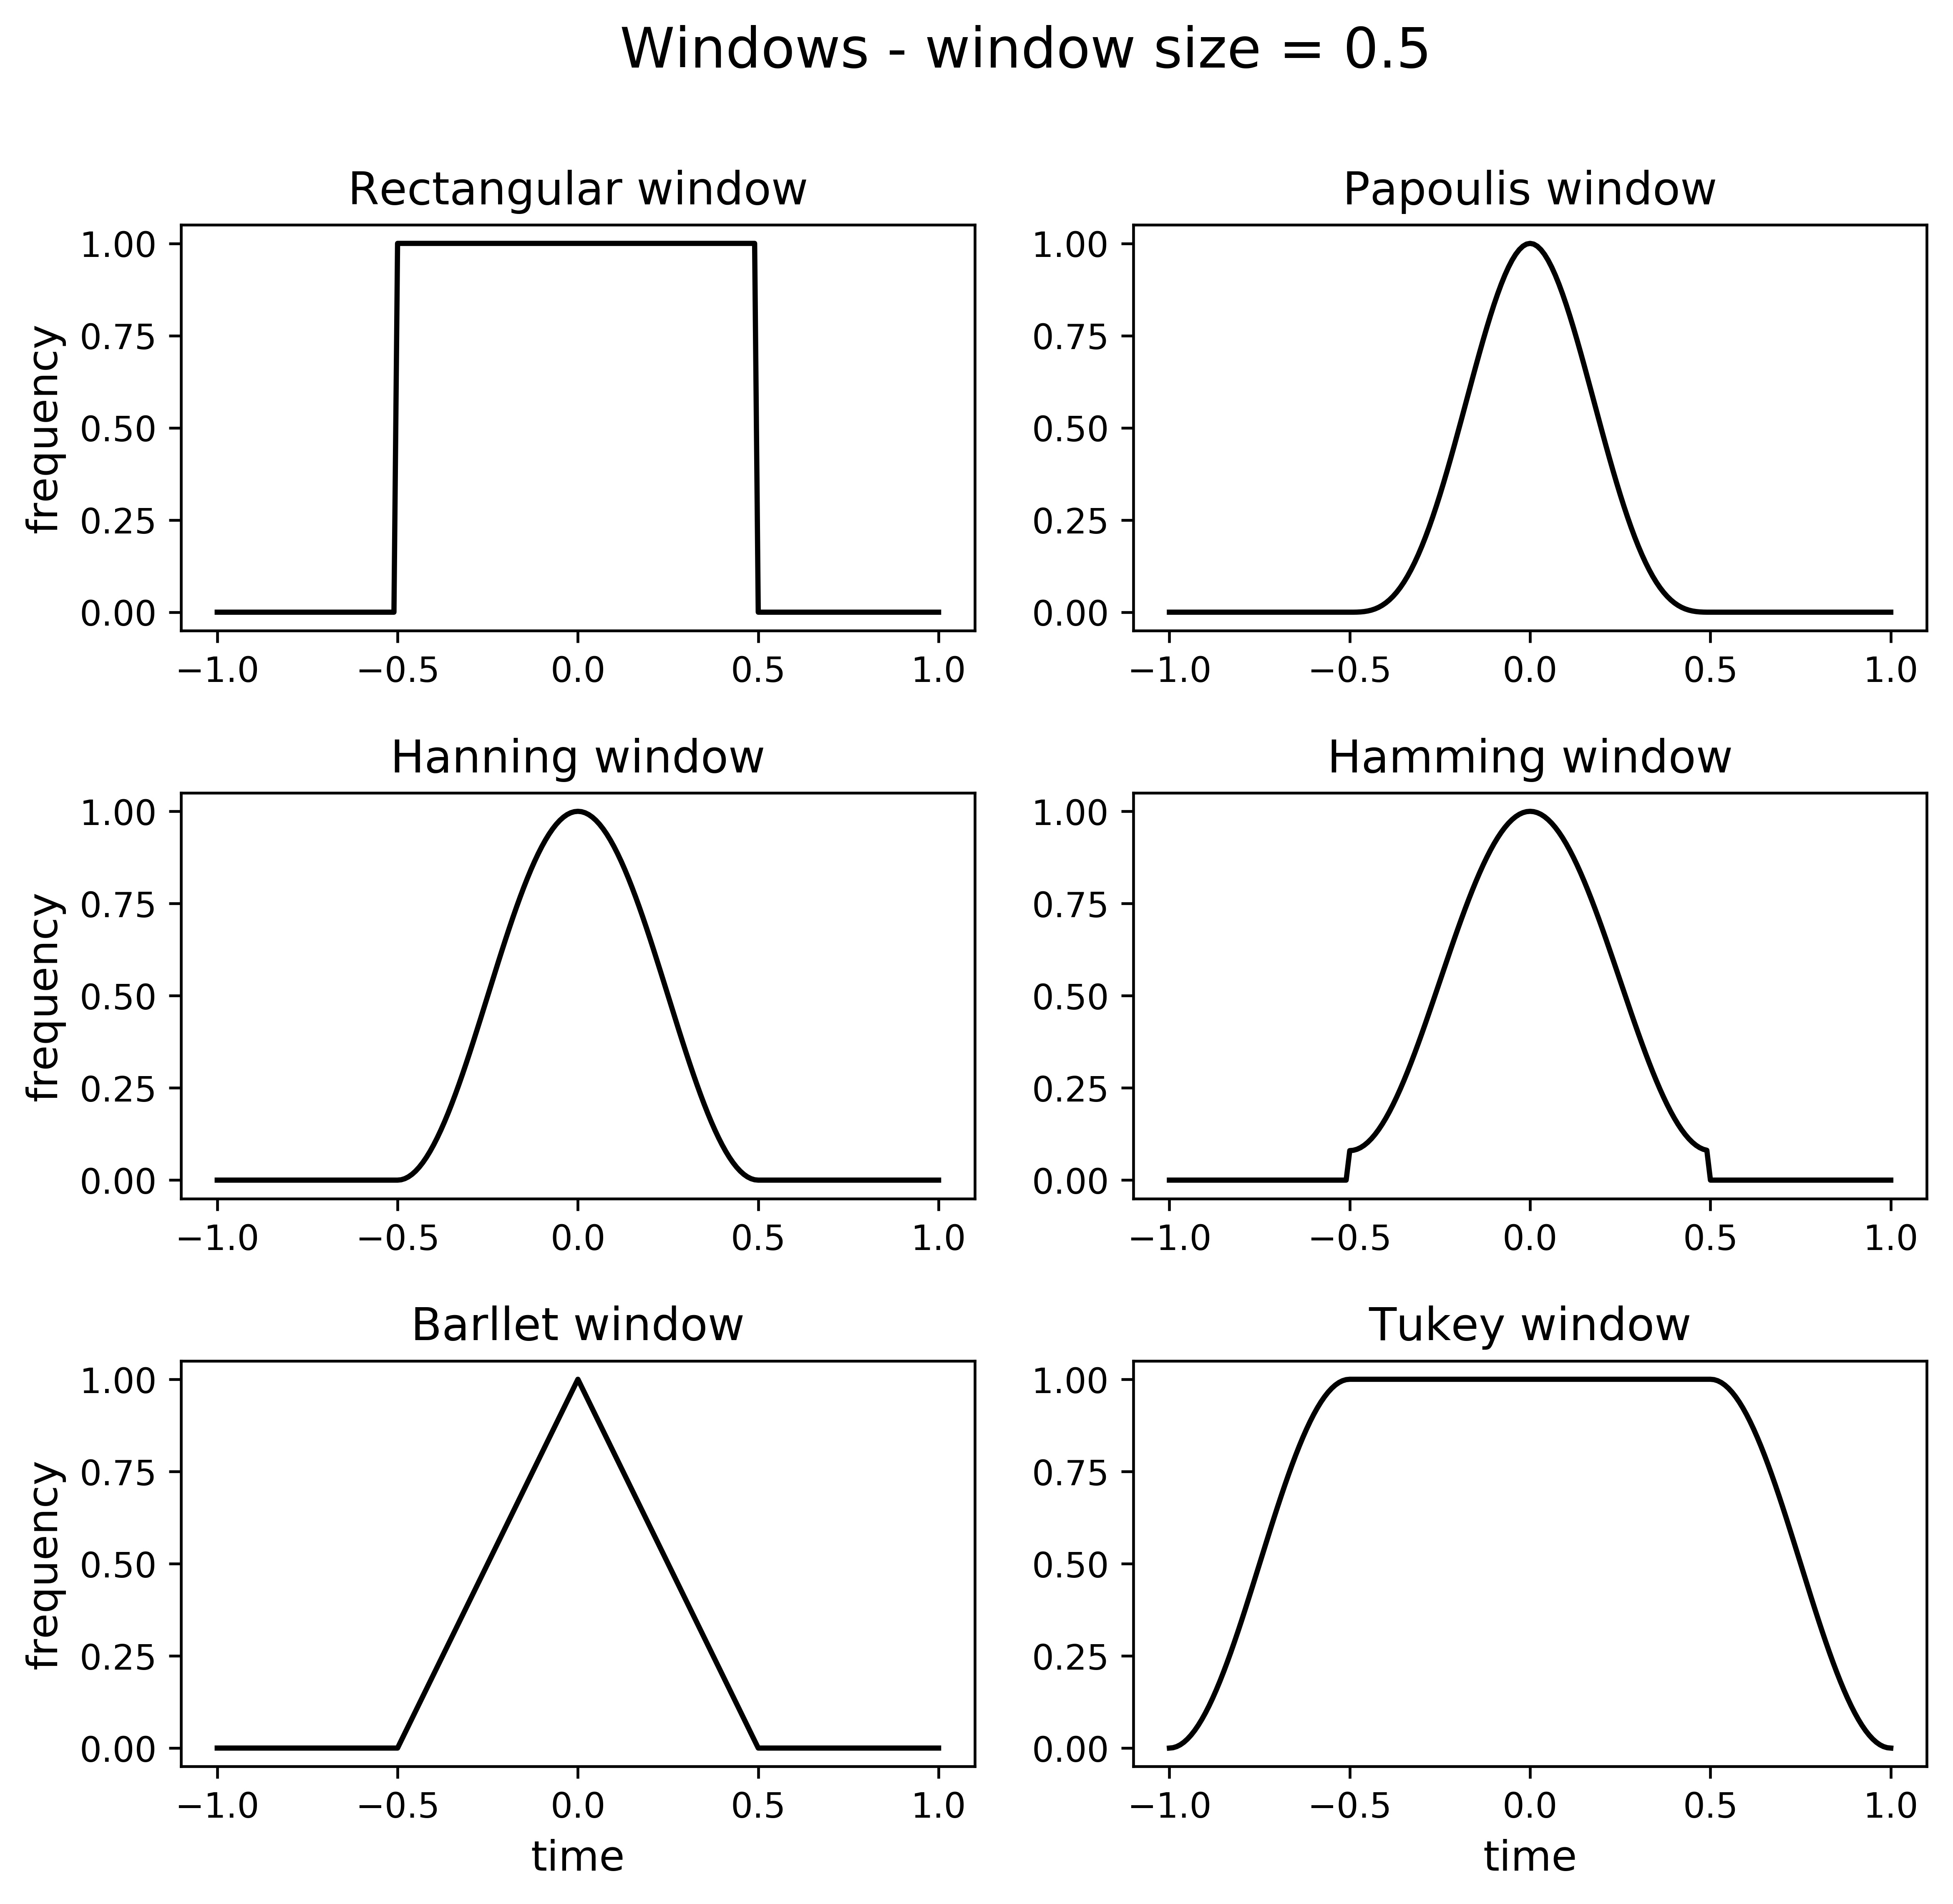
\includegraphics{../scripts/exercicio2/janelas/Windows_plots_ws0.5.jpg}}	
	\end{center}
	\vspace{1mm}	% acrescentar o espaçamento vertical apropriado entre a borda inferior da figura e a legenda ou a fonte quando não há legenda (o valor pode ser negativo para subir)
	%\legenda{Figura 1.1: Dez sinais e seus respectivos histogramas para  asérie com $N$ = 64 do grupo noise.}	% legenda - para deixar sem legenda usar comando \legenda{} (nunca deve-se comentar o comando \legenda)
	\label{ex1_fig1}
	%\FONTE{}	% fonte consultada (elemento obrigatório, mesmo que seja produção do próprio autor)
\end{figure}

% FIGURA
\begin{figure}[ht!]
	\legenda{Figura 2.2: Transformadas de Fourier das funções janela utilizadas neste exercício com largura igual a 0.5.}
	\vspace{2mm}	% acrescentar o espaçamento vertical apropriado entre o título e a borda superior da figura
	\begin{center}
		\resizebox{\textwidth}{!}{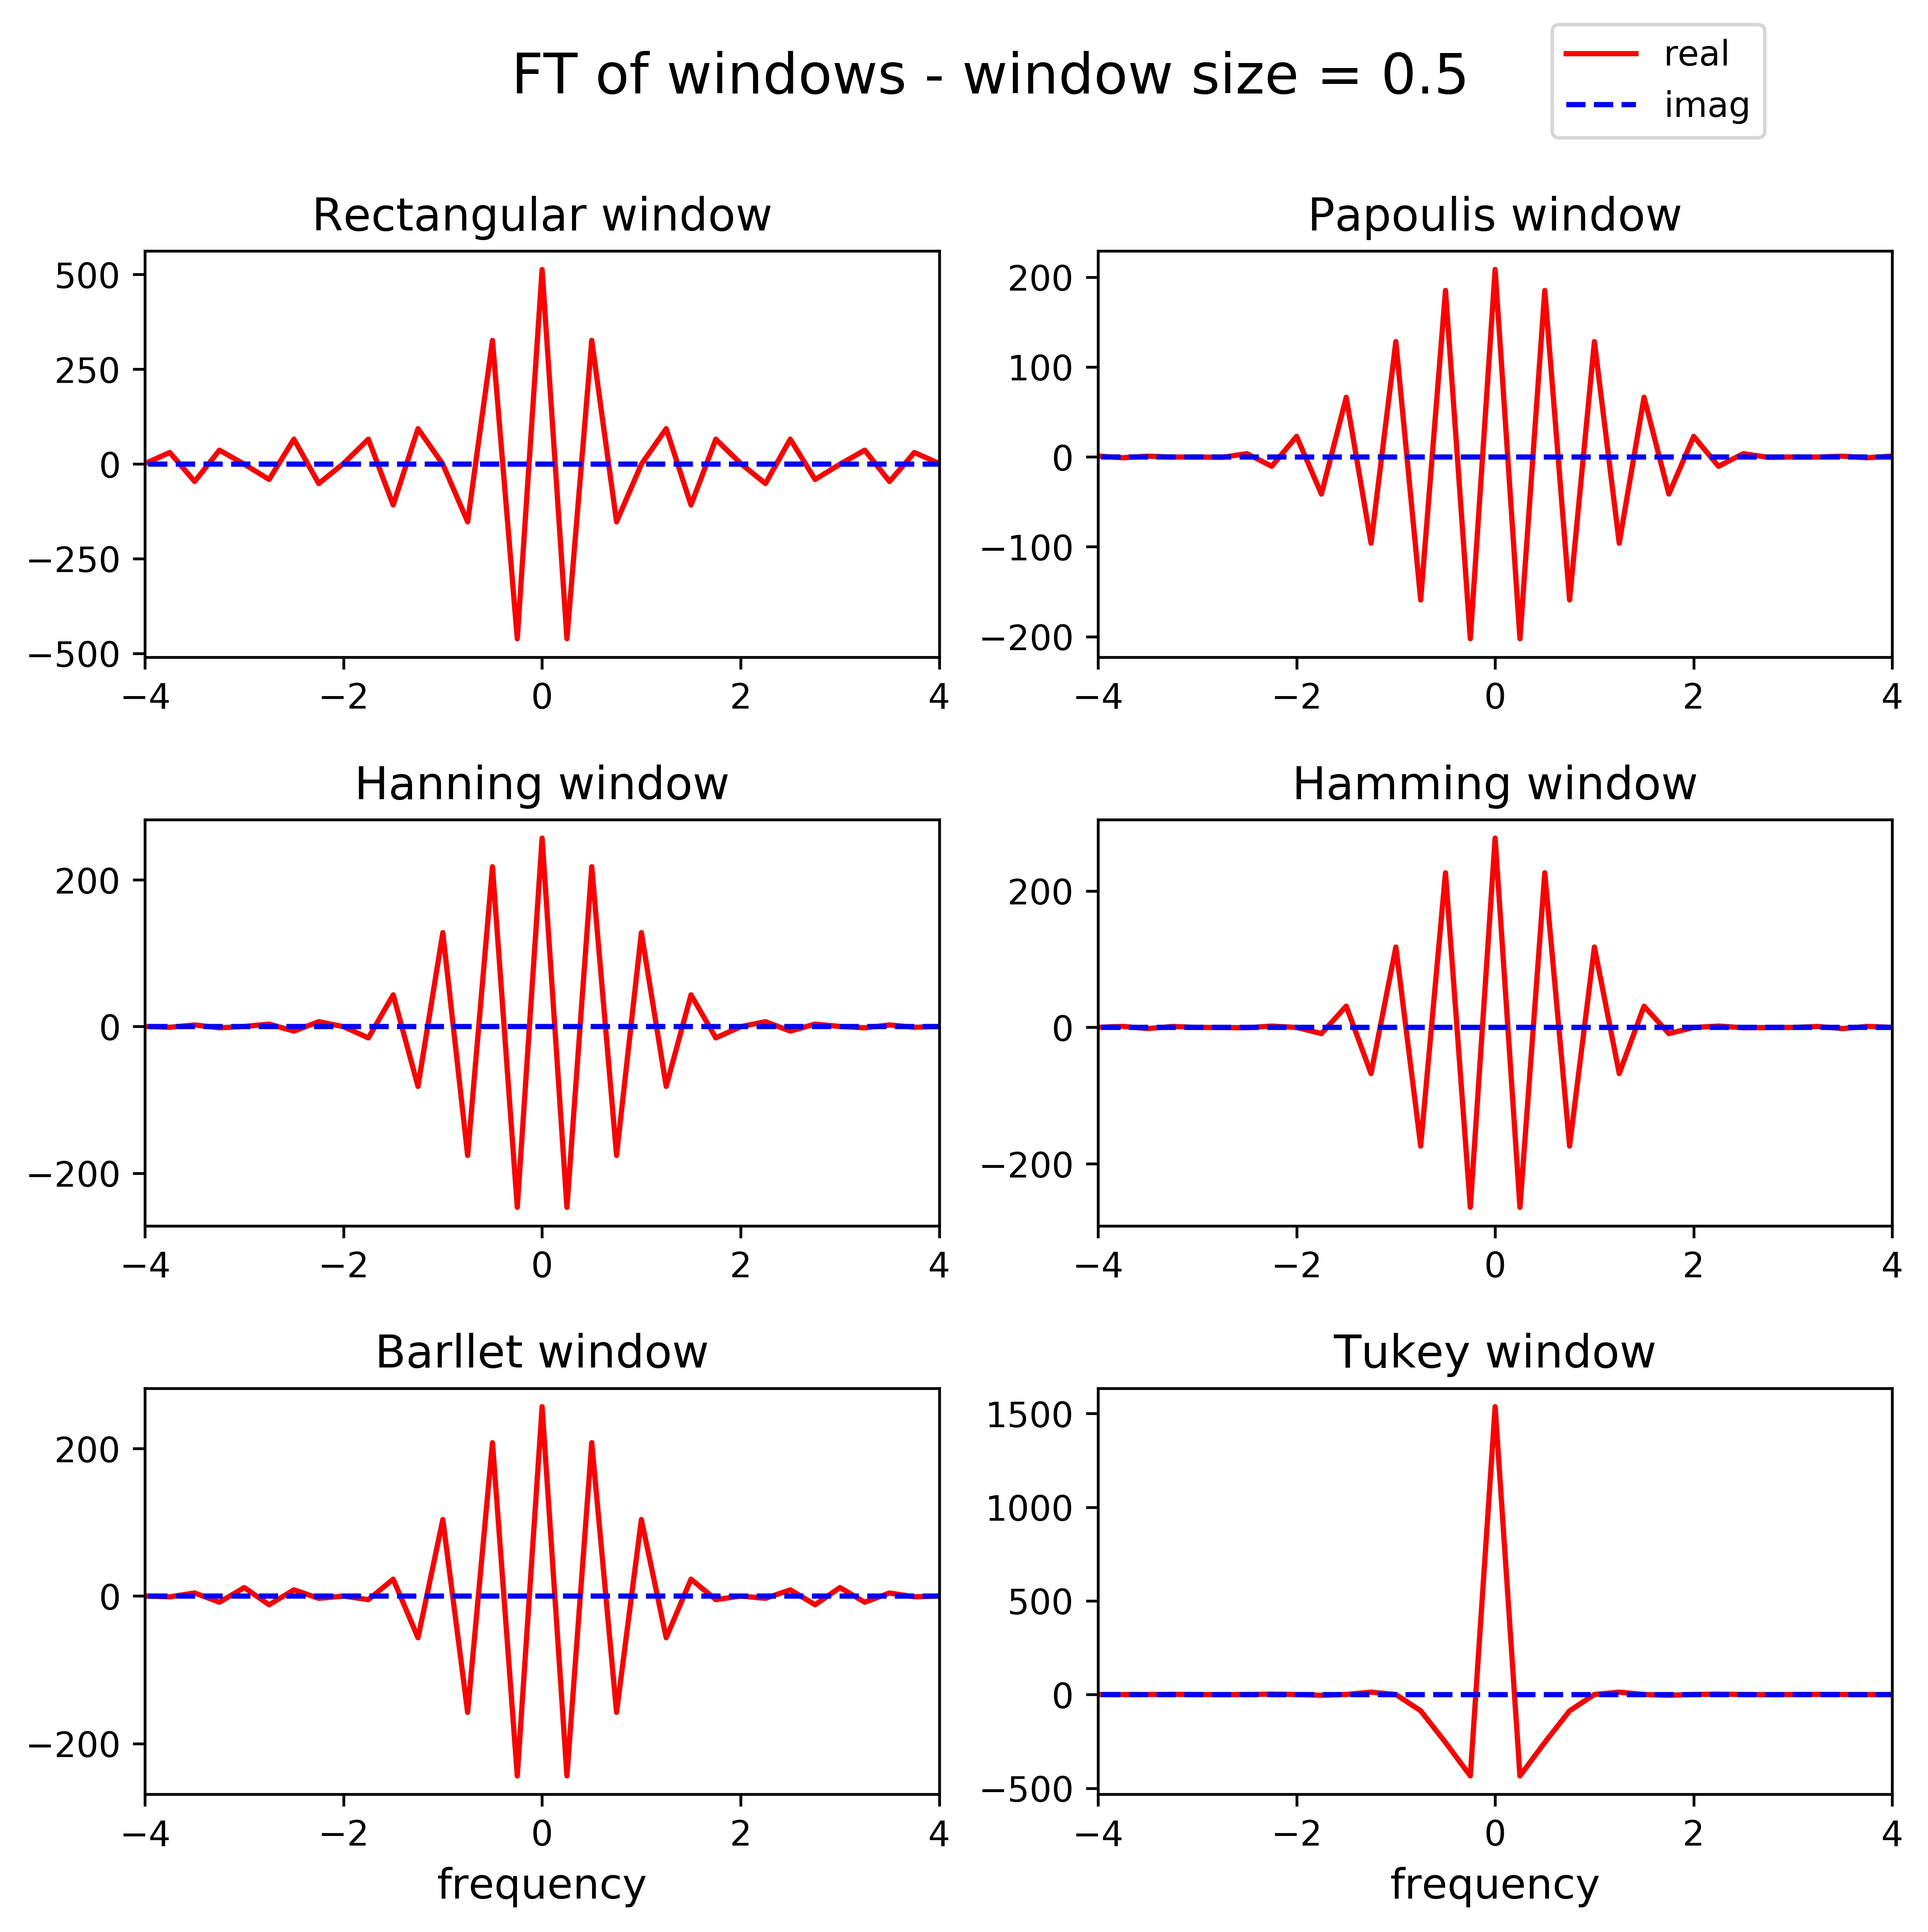
\includegraphics{../scripts/exercicio2/ffts/Windows_FFTs_ws0.5.jpg}}	
	\end{center}
	\vspace{1mm}	% acrescentar o espaçamento vertical apropriado entre a borda inferior da figura e a legenda ou a fonte quando não há legenda (o valor pode ser negativo para subir)
	%\legenda{Figura 1.1: Dez sinais e seus respectivos histogramas para  asérie com $N$ = 64 do grupo noise.}	% legenda - para deixar sem legenda usar comando \legenda{} (nunca deve-se comentar o comando \legenda)
	\label{ex1_fig1}
	%\FONTE{}	% fonte consultada (elemento obrigatório, mesmo que seja produção do próprio autor)
\end{figure}


As mesmas janelas, porém com tamanho igual a 0.1, produzem os resultados das Figuras 2.3 e 2.4. 


% FIGURA
\begin{figure}[ht!]
	\legenda{Figura 2.3: Gráfico das seis janelas utilizadas neste exercício com largura (abaixo denominado \texttt{window size}) igual a 0.1.}
	\vspace{2mm}	% acrescentar o espaçamento vertical apropriado entre o título e a borda superior da figura
	\begin{center}
		\resizebox{\textwidth}{!}{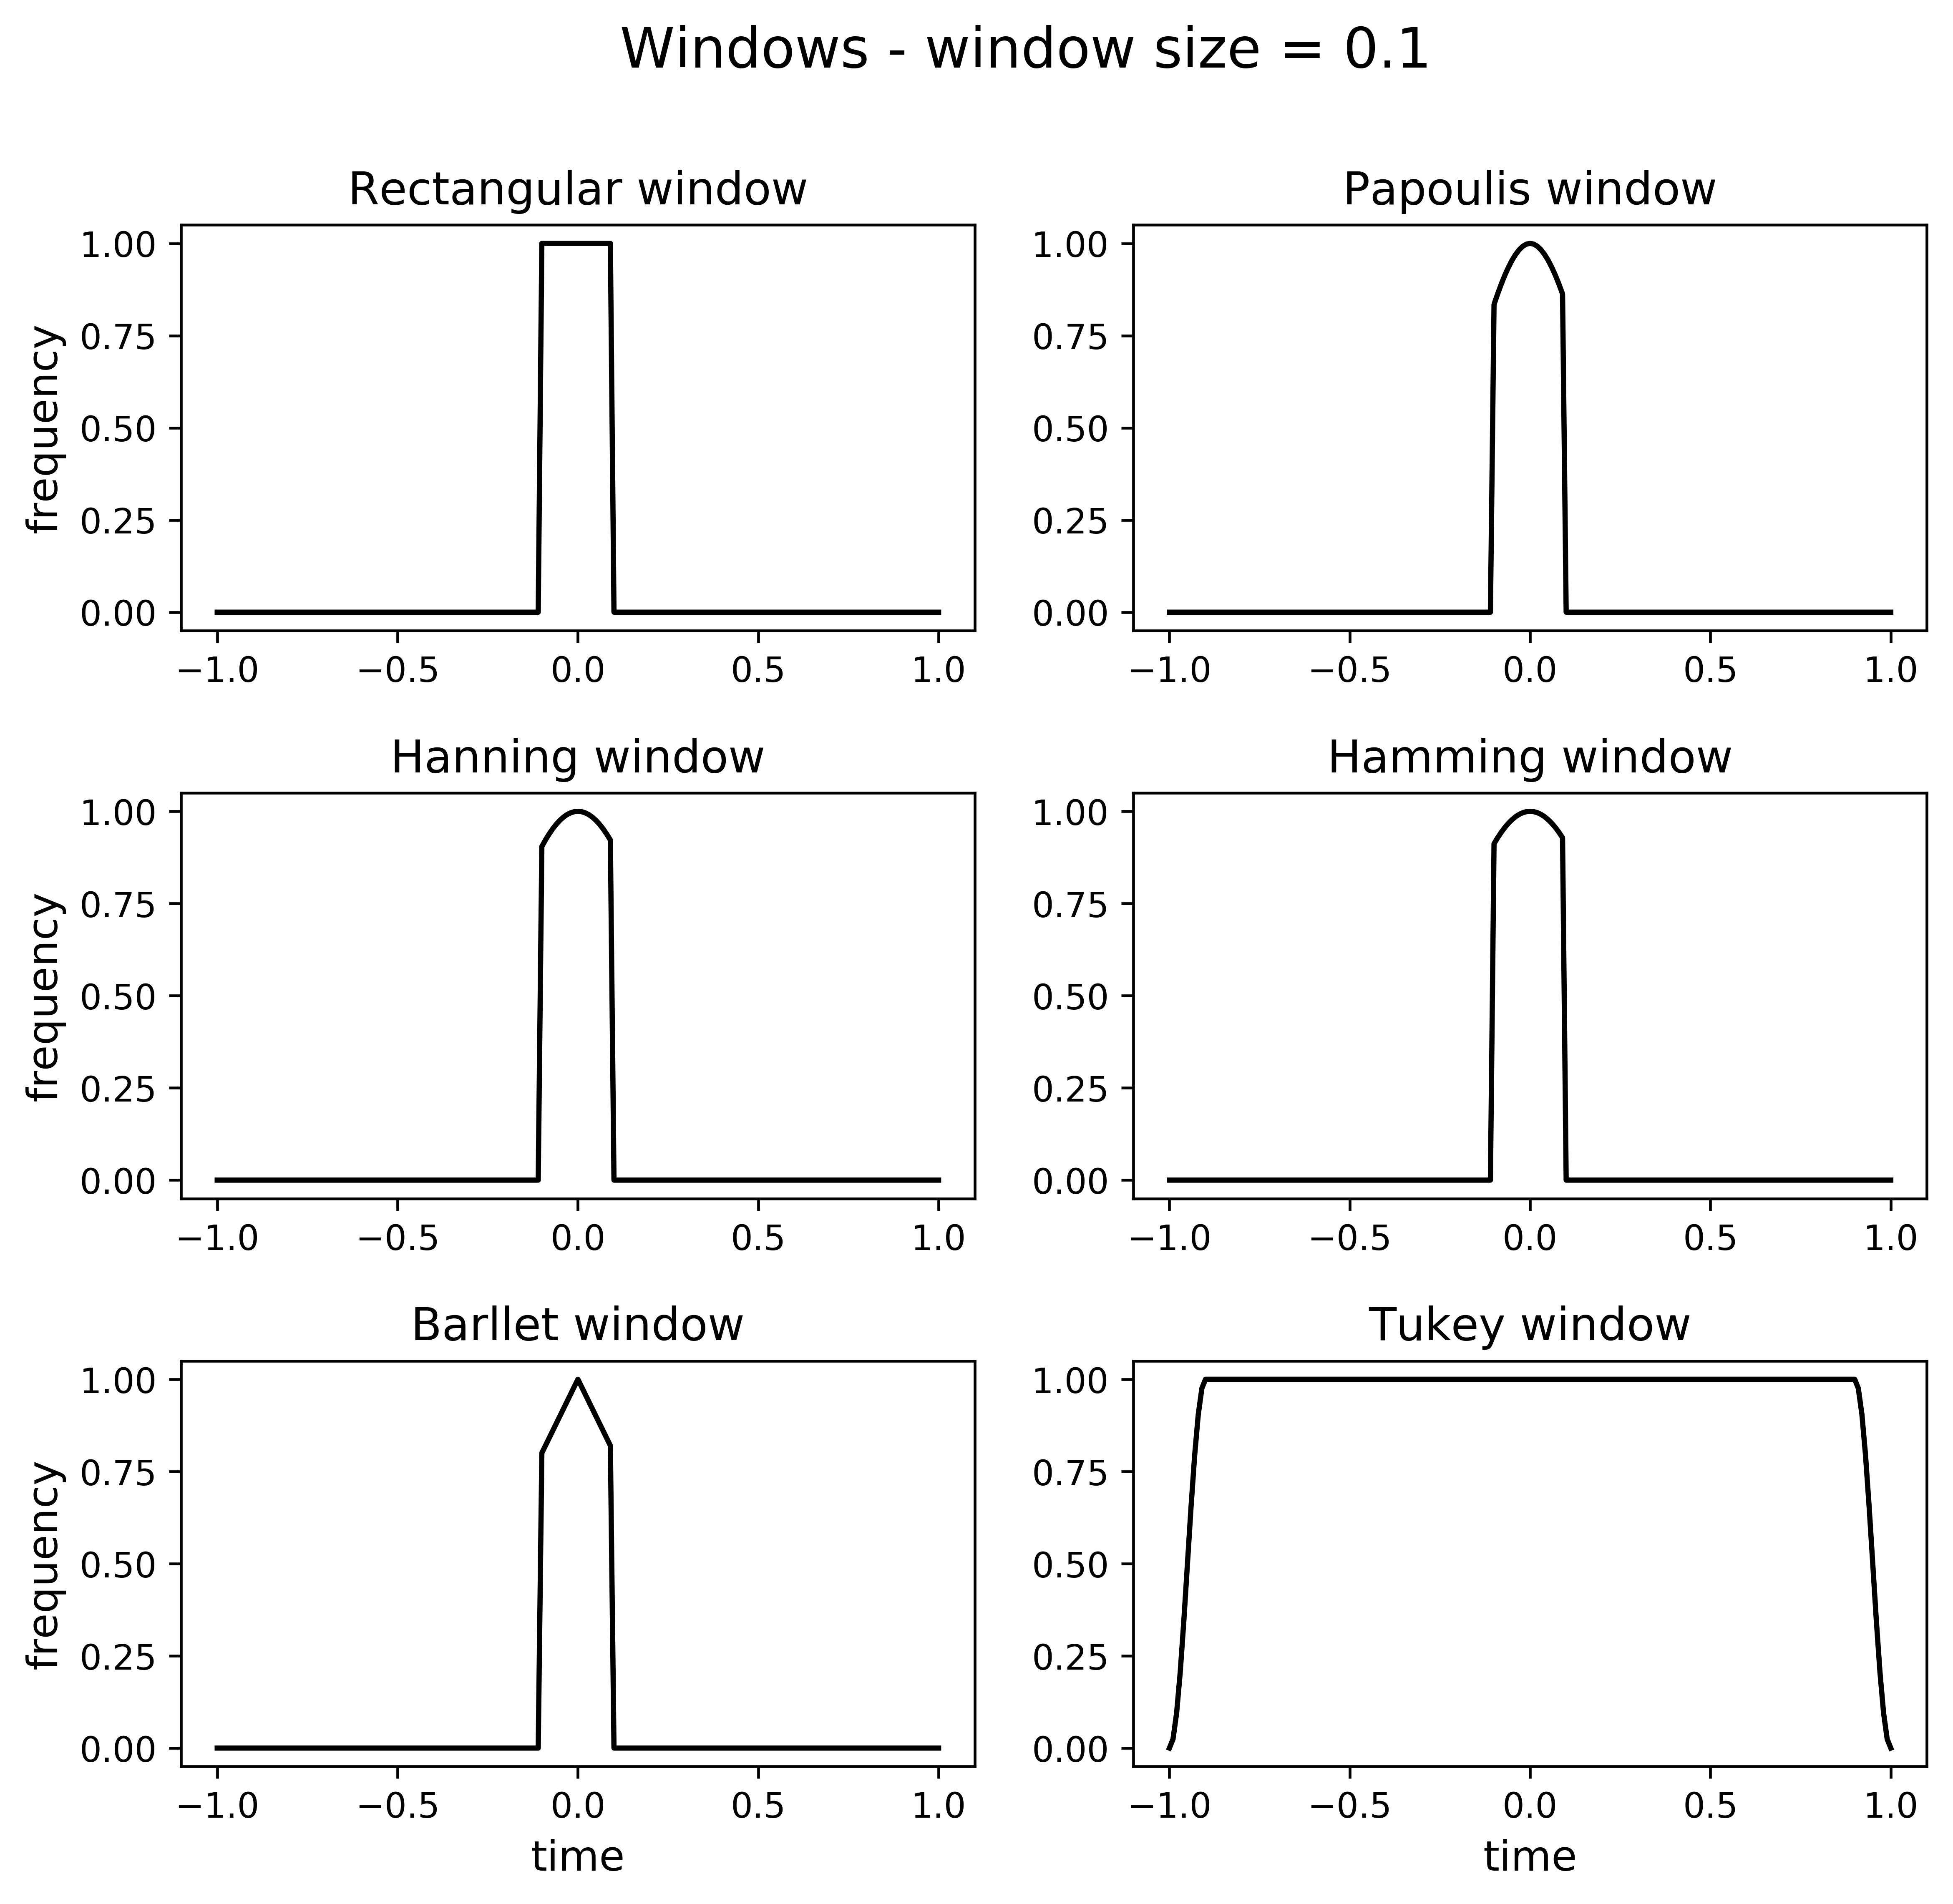
\includegraphics{../scripts/exercicio2/janelas/Windows_plots_ws0.1.jpg}}	
	\end{center}
	\vspace{1mm}	% acrescentar o espaçamento vertical apropriado entre a borda inferior da figura e a legenda ou a fonte quando não há legenda (o valor pode ser negativo para subir)
	%\legenda{Figura 1.1: Dez sinais e seus respectivos histogramas para  asérie com $N$ = 64 do grupo noise.}	% legenda - para deixar sem legenda usar comando \legenda{} (nunca deve-se comentar o comando \legenda)
	\label{ex1_fig1}
	%\FONTE{}	% fonte consultada (elemento obrigatório, mesmo que seja produção do próprio autor)
\end{figure}

% FIGURA
\begin{figure}[ht!]
	\legenda{Figura 2.4: Transformadas de Fourier das funções janela utilizadas neste exercício com largura igual a 0.1.}
	\vspace{2mm}	% acrescentar o espaçamento vertical apropriado entre o título e a borda superior da figura
	\begin{center}
		\resizebox{\textwidth}{!}{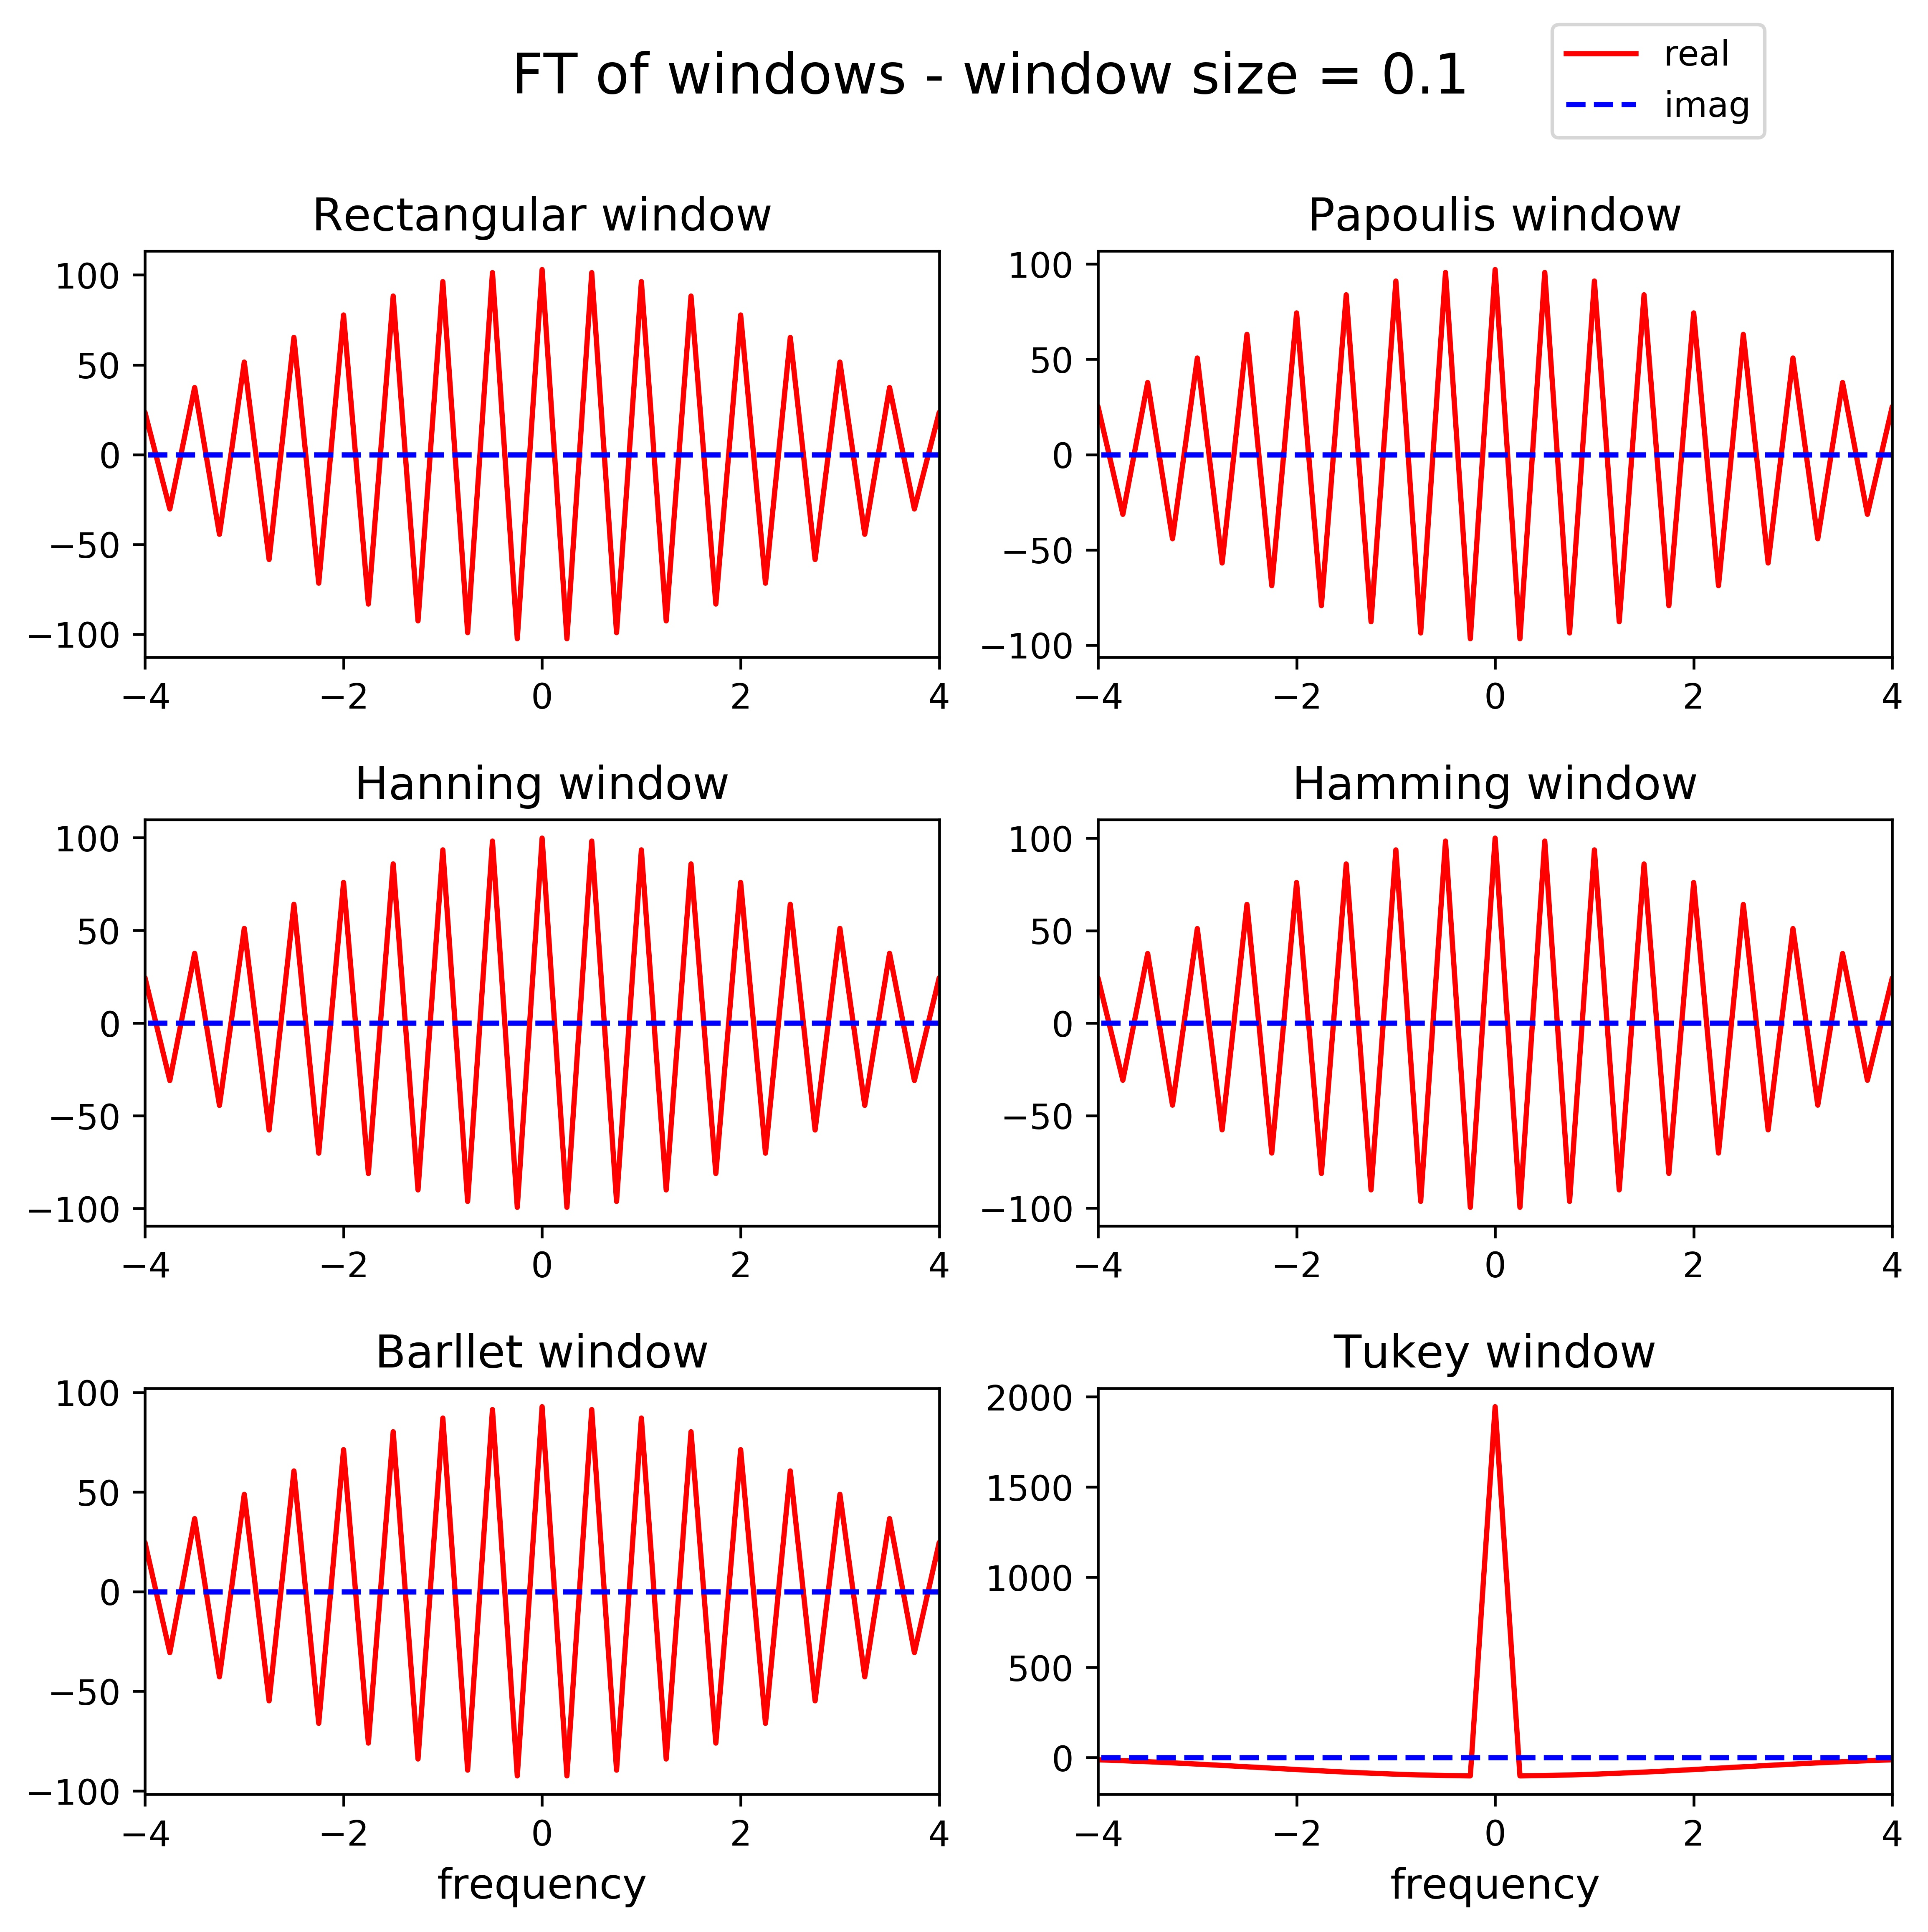
\includegraphics{../scripts/exercicio2/ffts/Windows_FFTs_ws0.1.jpg}}	
	\end{center}
	\vspace{1mm}	% acrescentar o espaçamento vertical apropriado entre a borda inferior da figura e a legenda ou a fonte quando não há legenda (o valor pode ser negativo para subir)
	%\legenda{Figura 1.1: Dez sinais e seus respectivos histogramas para  asérie com $N$ = 64 do grupo noise.}	% legenda - para deixar sem legenda usar comando \legenda{} (nunca deve-se comentar o comando \legenda)
	\label{ex1_fig1}
	%\FONTE{}	% fonte consultada (elemento obrigatório, mesmo que seja produção do próprio autor)
\end{figure}


%%%%%%%%%%%%%%%%%%%%%%%%%%%%%%%%%%%%%%%%%%%%%%%%%%%%%%%%%% 2.b

\clearpage
\subsection*{2.b} 
\addcontentsline{toc}{section}{\protect\numberline{} 2.b}%

Dada uma escolha do sinal (variável \texttt{chirp} abaixo, à qual é atribuída um dos chirps do Exercício 1), os espectrogramas foram calculados a partir do método \texttt{spec}, recebendo como input: o produto do chirp e da função janela \textit{shiftada}, a resolução \texttt{res} (para cálculo dos bins de frequência), a frequência final de interesse \texttt{f\_final}, e o número de bins \texttt{N} com o qual a FFT será implementada.

\lstinputlisting[language=python, style=mystyle, firstline=298, lastline=348]{../scripts/exercicio2/espectros/window_spectra.py}

A seguir são apresentados os resultados das WFT de cada chirp do Exercício 1. Dois valores foram usados para o tamanho das janelas implementadas e dois domínios diferentes para cada chirp (a saber, os domínios referentes às Figuras 1.1 e 1.2). O espectrograma de cada caso foi gerado.

As figuras dos espectrogramas foram criadas com o pacote \texttt{matplotlib}, em particular com a função \texttt{countourf}. Foi utilizando o mapa de cor \texttt{jet} e 256 níveis de cor. Cada figura possui o mesmo intervalo de cor em sua representação (mesmos \texttt{vmin} e \texttt{vmax}). O trecho do código que gera a visualização das Figuras 2.4 a 2.16 é exibido abaixo:
\lstinputlisting[language=python, style=mystyle, firstline=352, lastline=411]{../scripts/exercicio2/espectros/window_spectra.py}

%%%%%%%%%%%%%%%% Gaussiano


Espectrogramas do \textbf{chirp gaussiano}, $-2 \leq t \leq 2$ e tamanho das janelas = 0.1: Figura 2.4.

% FIGURA
\begin{figure}[ht!]
	\legenda{Figura 2.4: Espectrogramas do chirp gaussiano com as seis funções janela usadas neste exercício de tamanho (largura) igual a 0.1. Comparar com o topo da Figura 1.1.}
	\vspace{3mm}	
	\begin{center}
		\resizebox{\textwidth}{!}{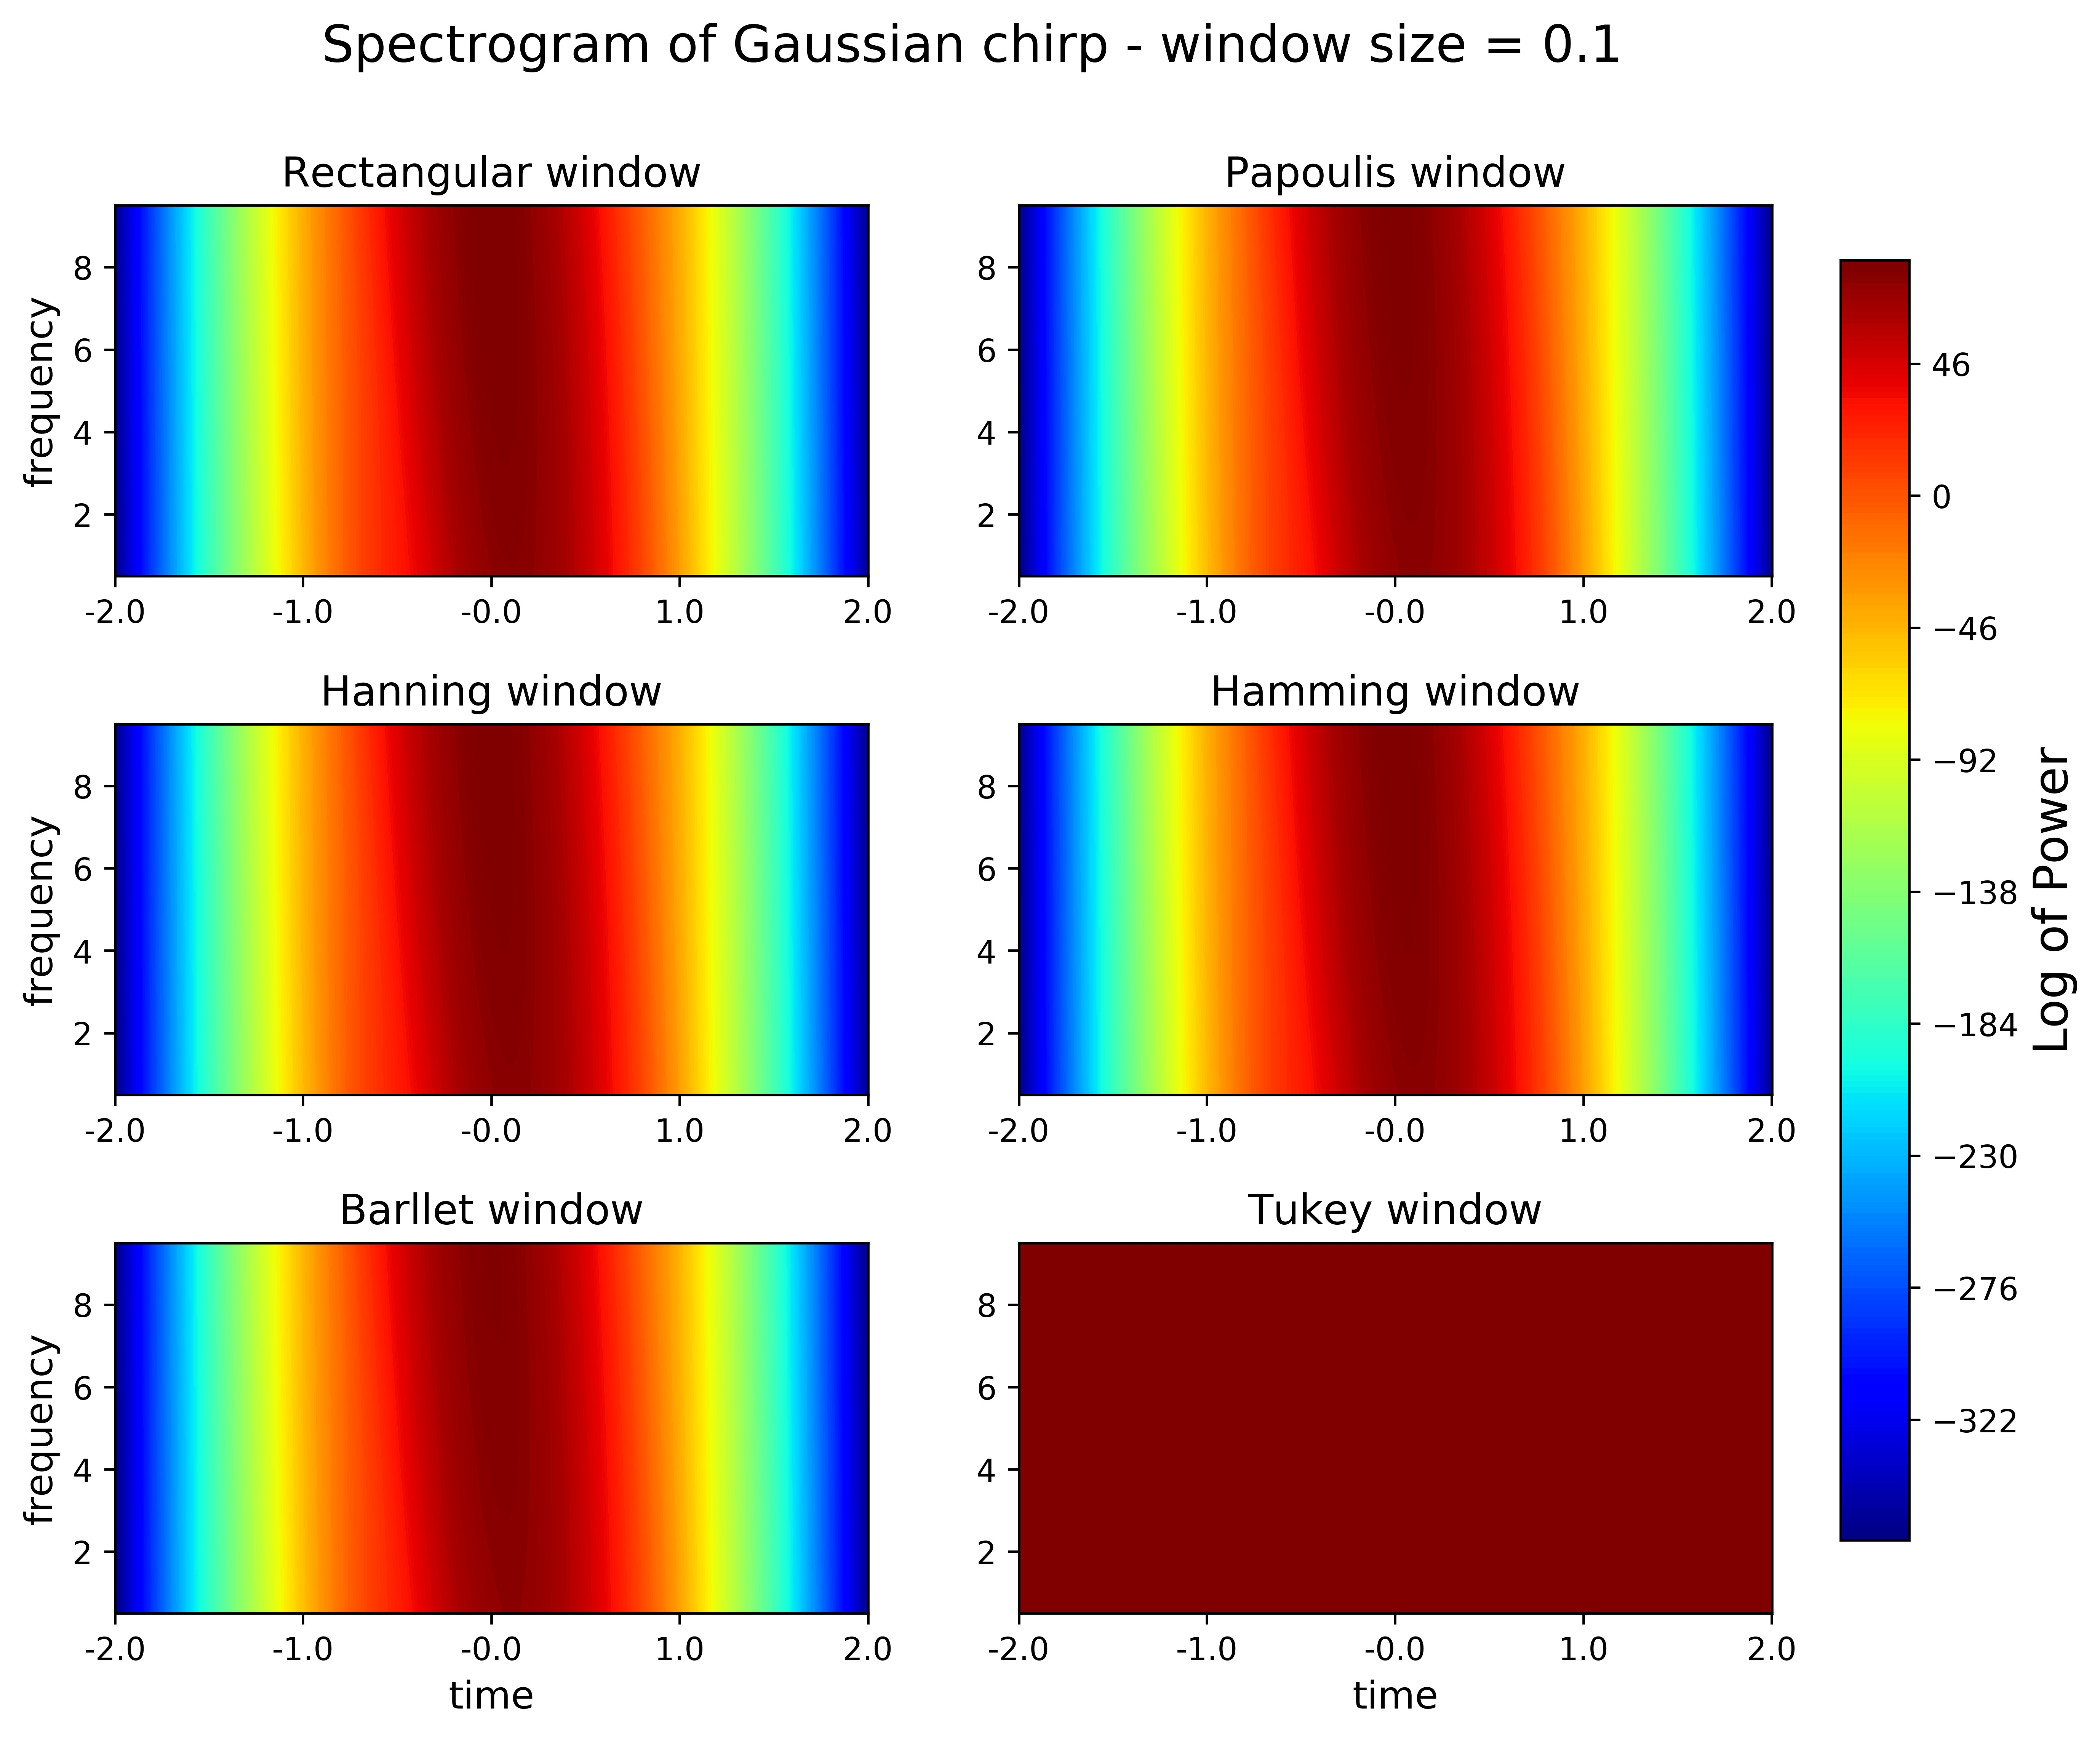
\includegraphics{../scripts/exercicio2/espectros/Gaussian_ws0.1.jpg}}	
	\end{center}
	\vspace{1mm}	
	\label{ex1_fig1}
\end{figure}

Espectrogramas do \textbf{chirp gaussiano}, $-2 \leq t \leq 2$ e tamanho das janelas = 0.5: Figura 2.5.

% FIGURA
\begin{figure}[ht!]
	\legenda{Figura 2.5: Espectrogramas do chirp gaussiano com as seis funções janela usadas neste exercício de tamanho (largura) igual a 0.5. Comparar com o topo da Figura 1.1.}
	\vspace{3mm}	
	\begin{center}
		\resizebox{\textwidth}{!}{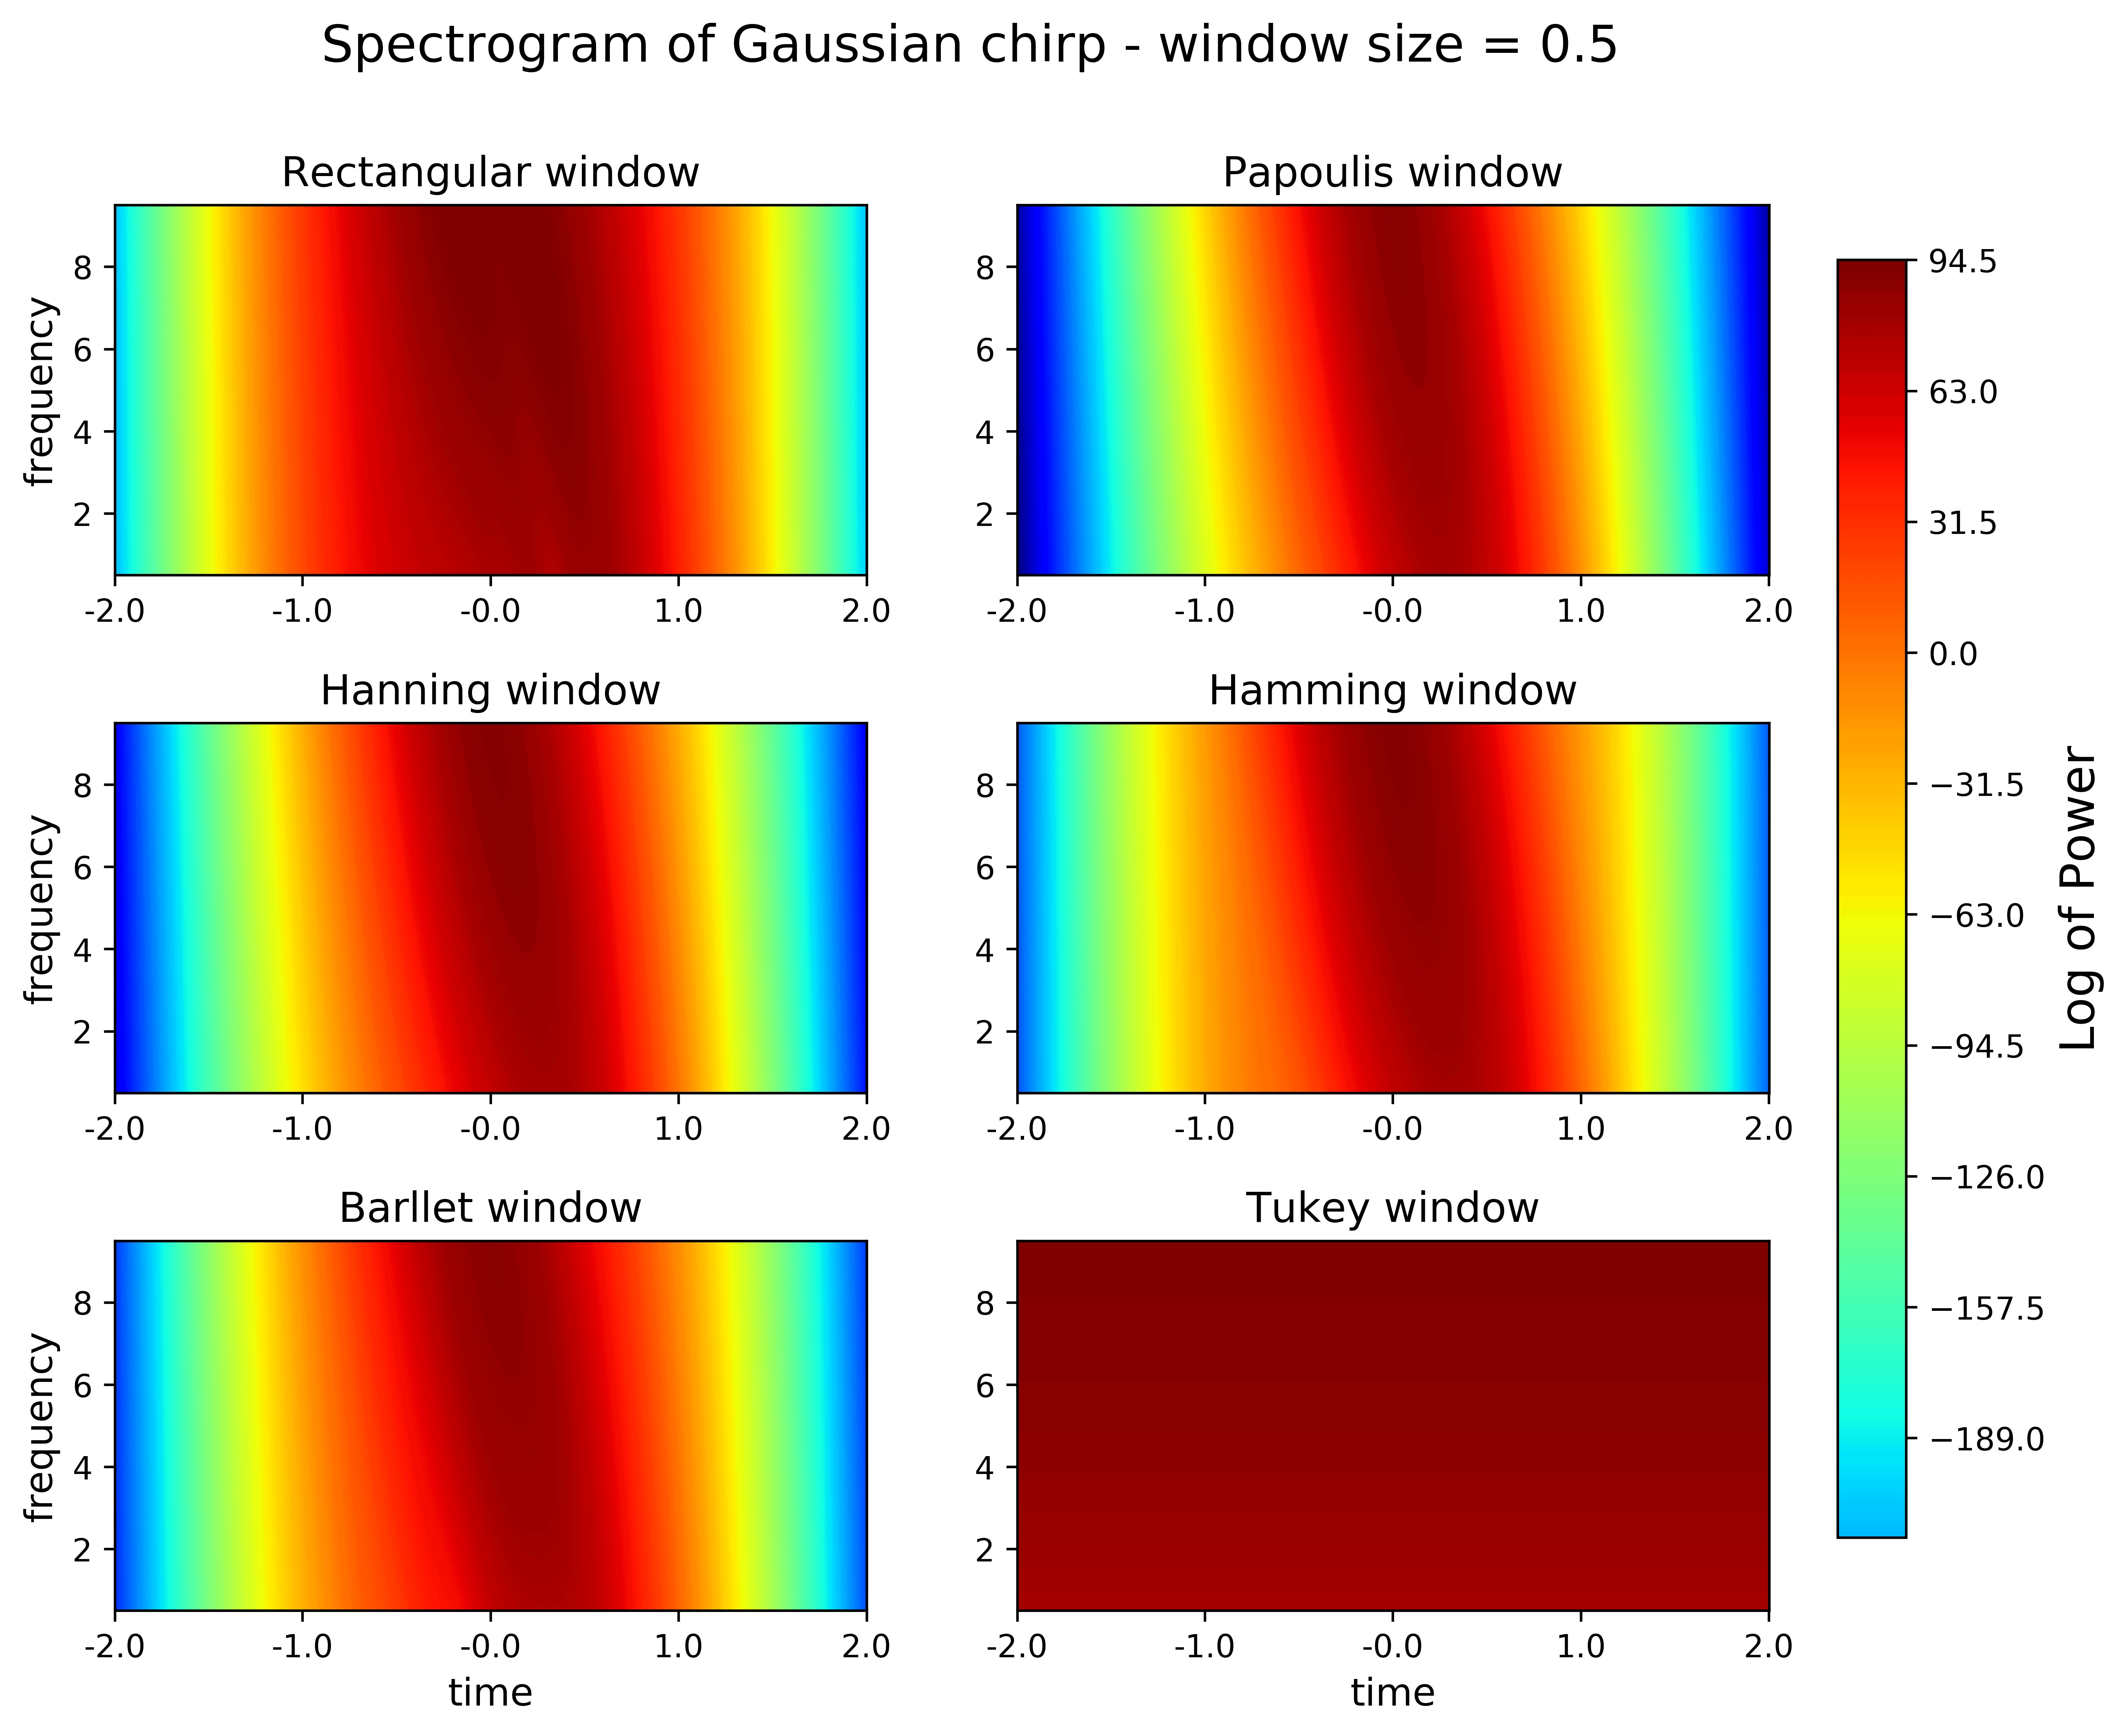
\includegraphics{../scripts/exercicio2/espectros/Gaussian_ws0.5.jpg}}	
	\end{center}
	\vspace{1mm}
	\label{ex1_fig1}
\end{figure}


Espectrogramas do \textbf{chirp gaussiano}, $0 \leq t \leq 6$ e tamanho das janelas = 0.5: Figura 2.6.

% FIGURA
\begin{figure}[ht!]
	\legenda{Figura 2.6: Espectrogramas do chirp gaussiano com as seis funções janela usadas neste exercício de tamanho (largura) igual a 0.5. Comparar com o topo da Figura 1.3.}
	\vspace{3mm}	
	\begin{center}
		\resizebox{\textwidth}{!}{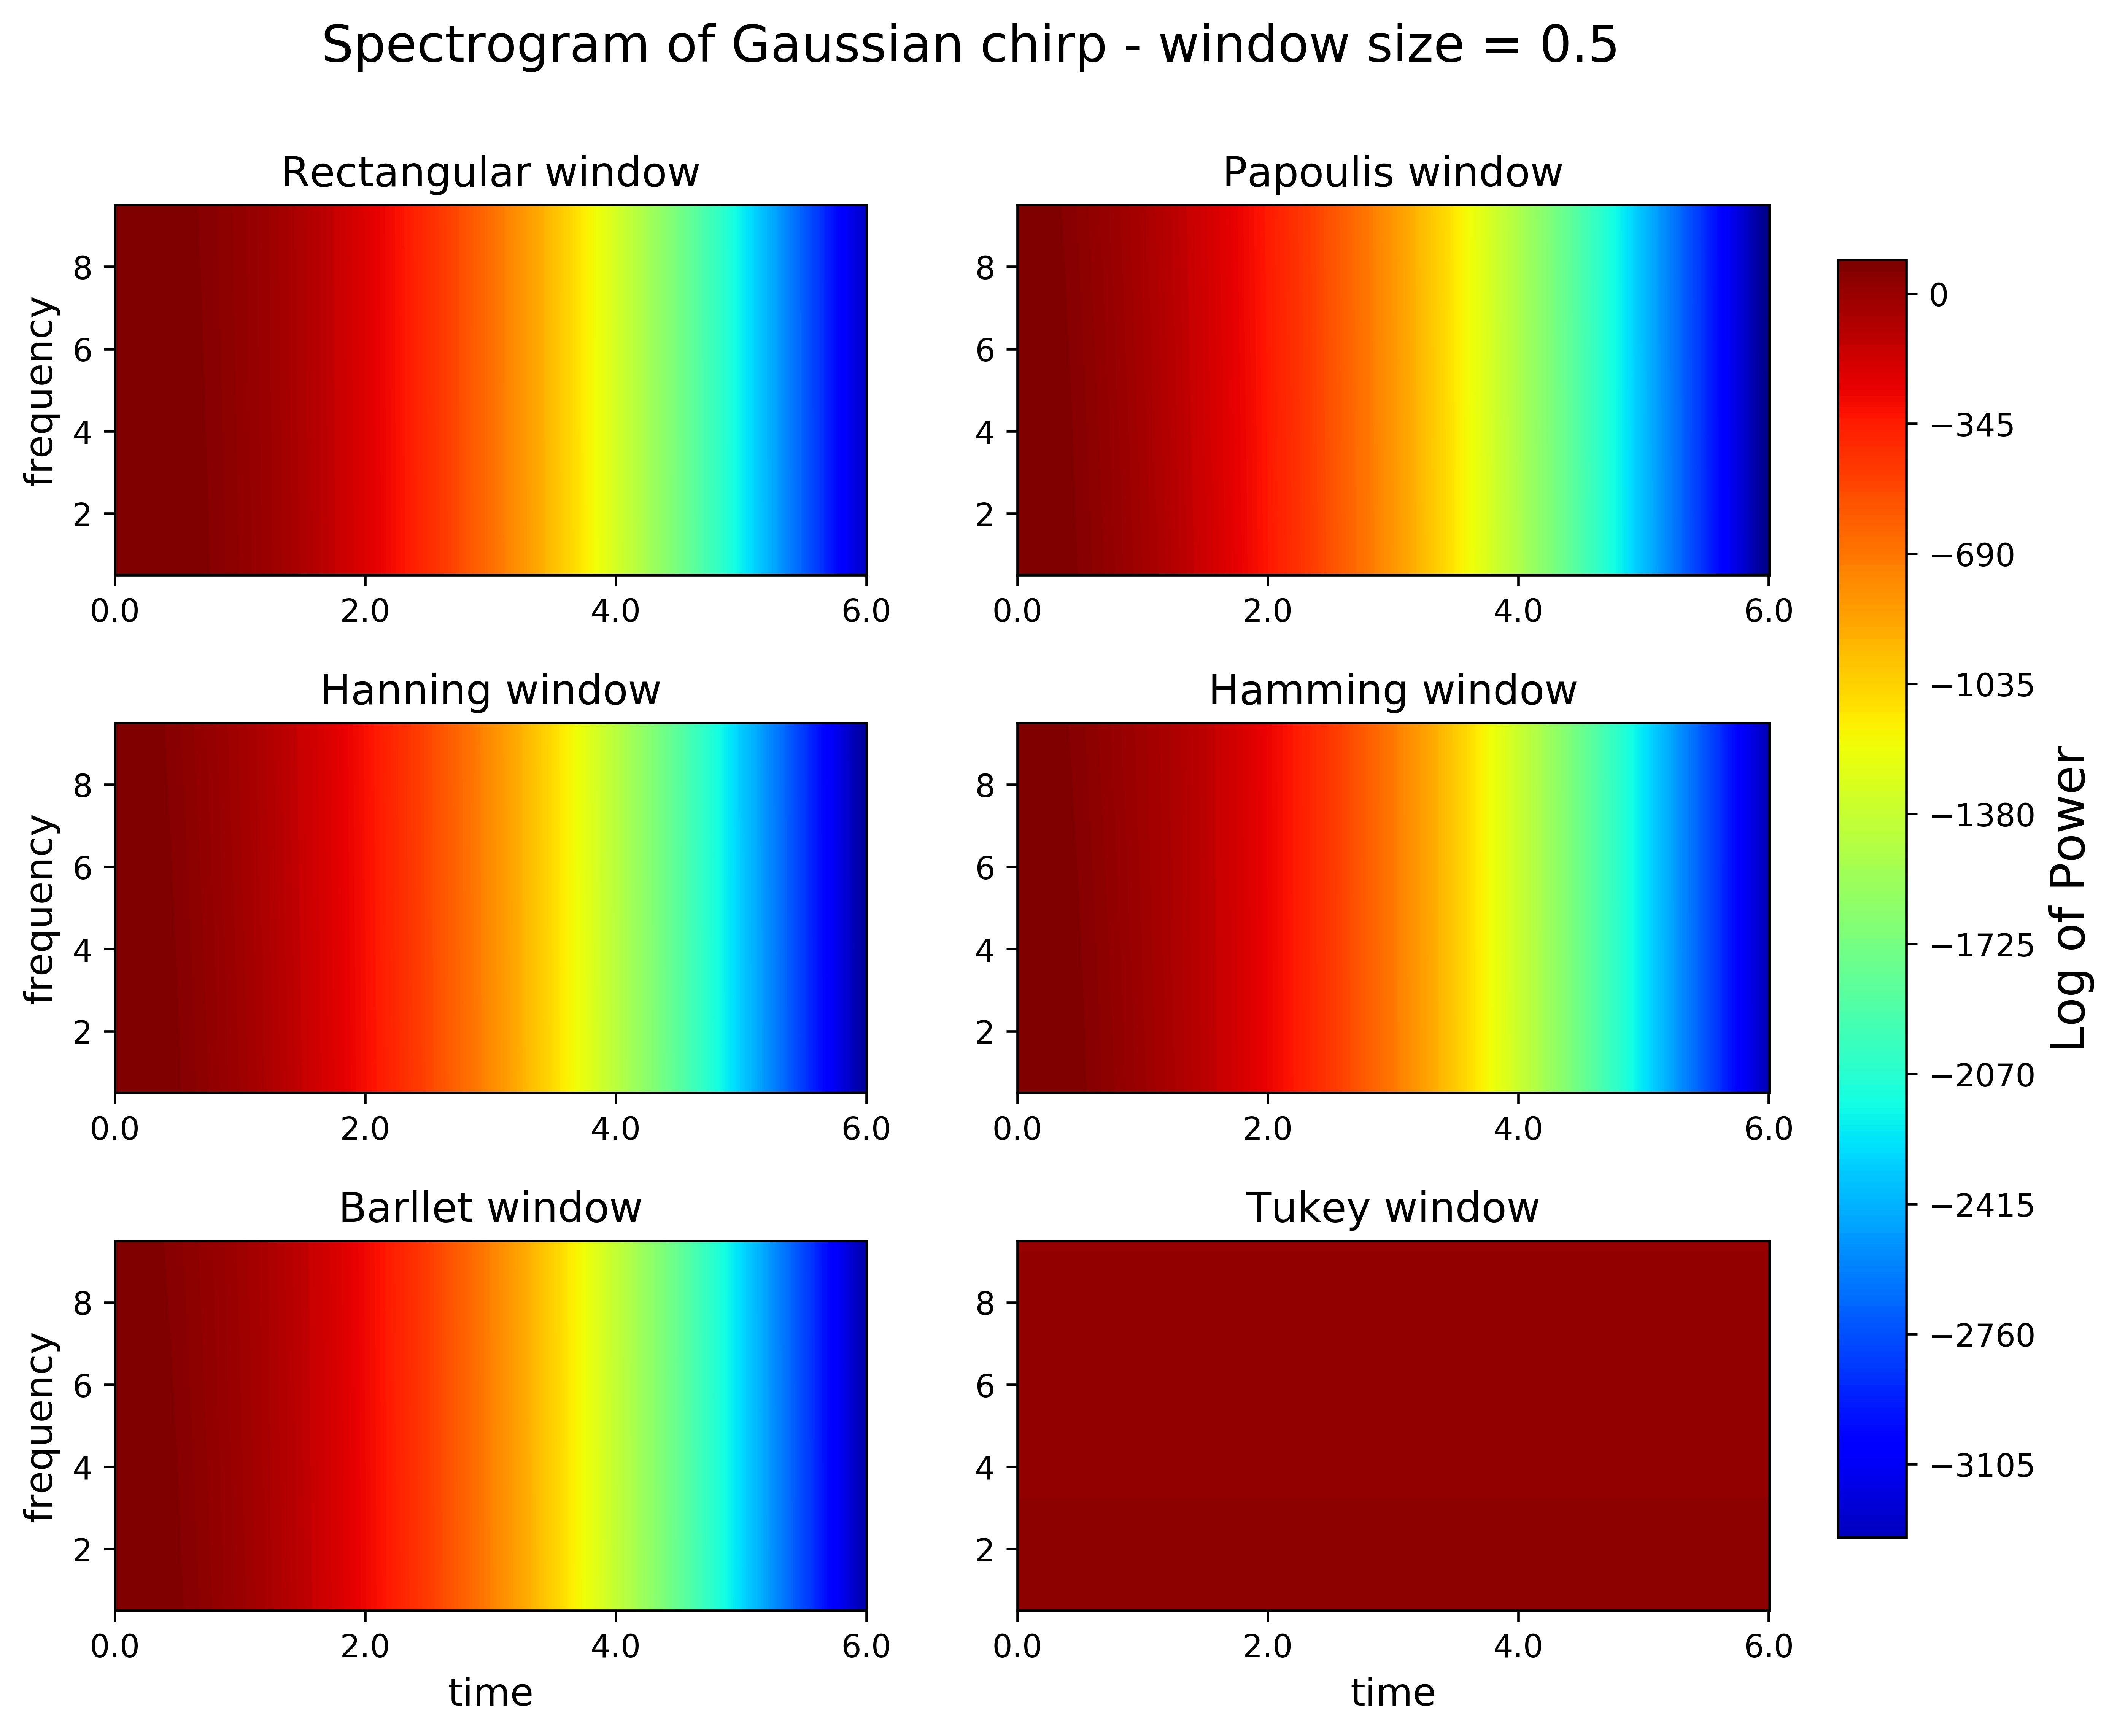
\includegraphics{../scripts/exercicio2/espectros/TEST_Gaussian_ws0.5.jpg}}	
	\end{center}
	\vspace{1mm}
	\label{ex1_fig1}
\end{figure}


%%%%%%%%%%%%%%%% Linear


Espectrogramas do \textbf{chirp linear}, $-6 \leq t \leq 6$ e tamanho das janelas = 0.1: Figura 2.7.

% FIGURA
\begin{figure}[ht!]
	\legenda{Figura 2.7: Espectrogramas do chirp linear com janelas de tamanho igual a 0.1. Comparar com segunda linha (de cima para baixo) da Figura 1.1.}
	\vspace{3mm}	
	\begin{center}
		\resizebox{\textwidth}{!}{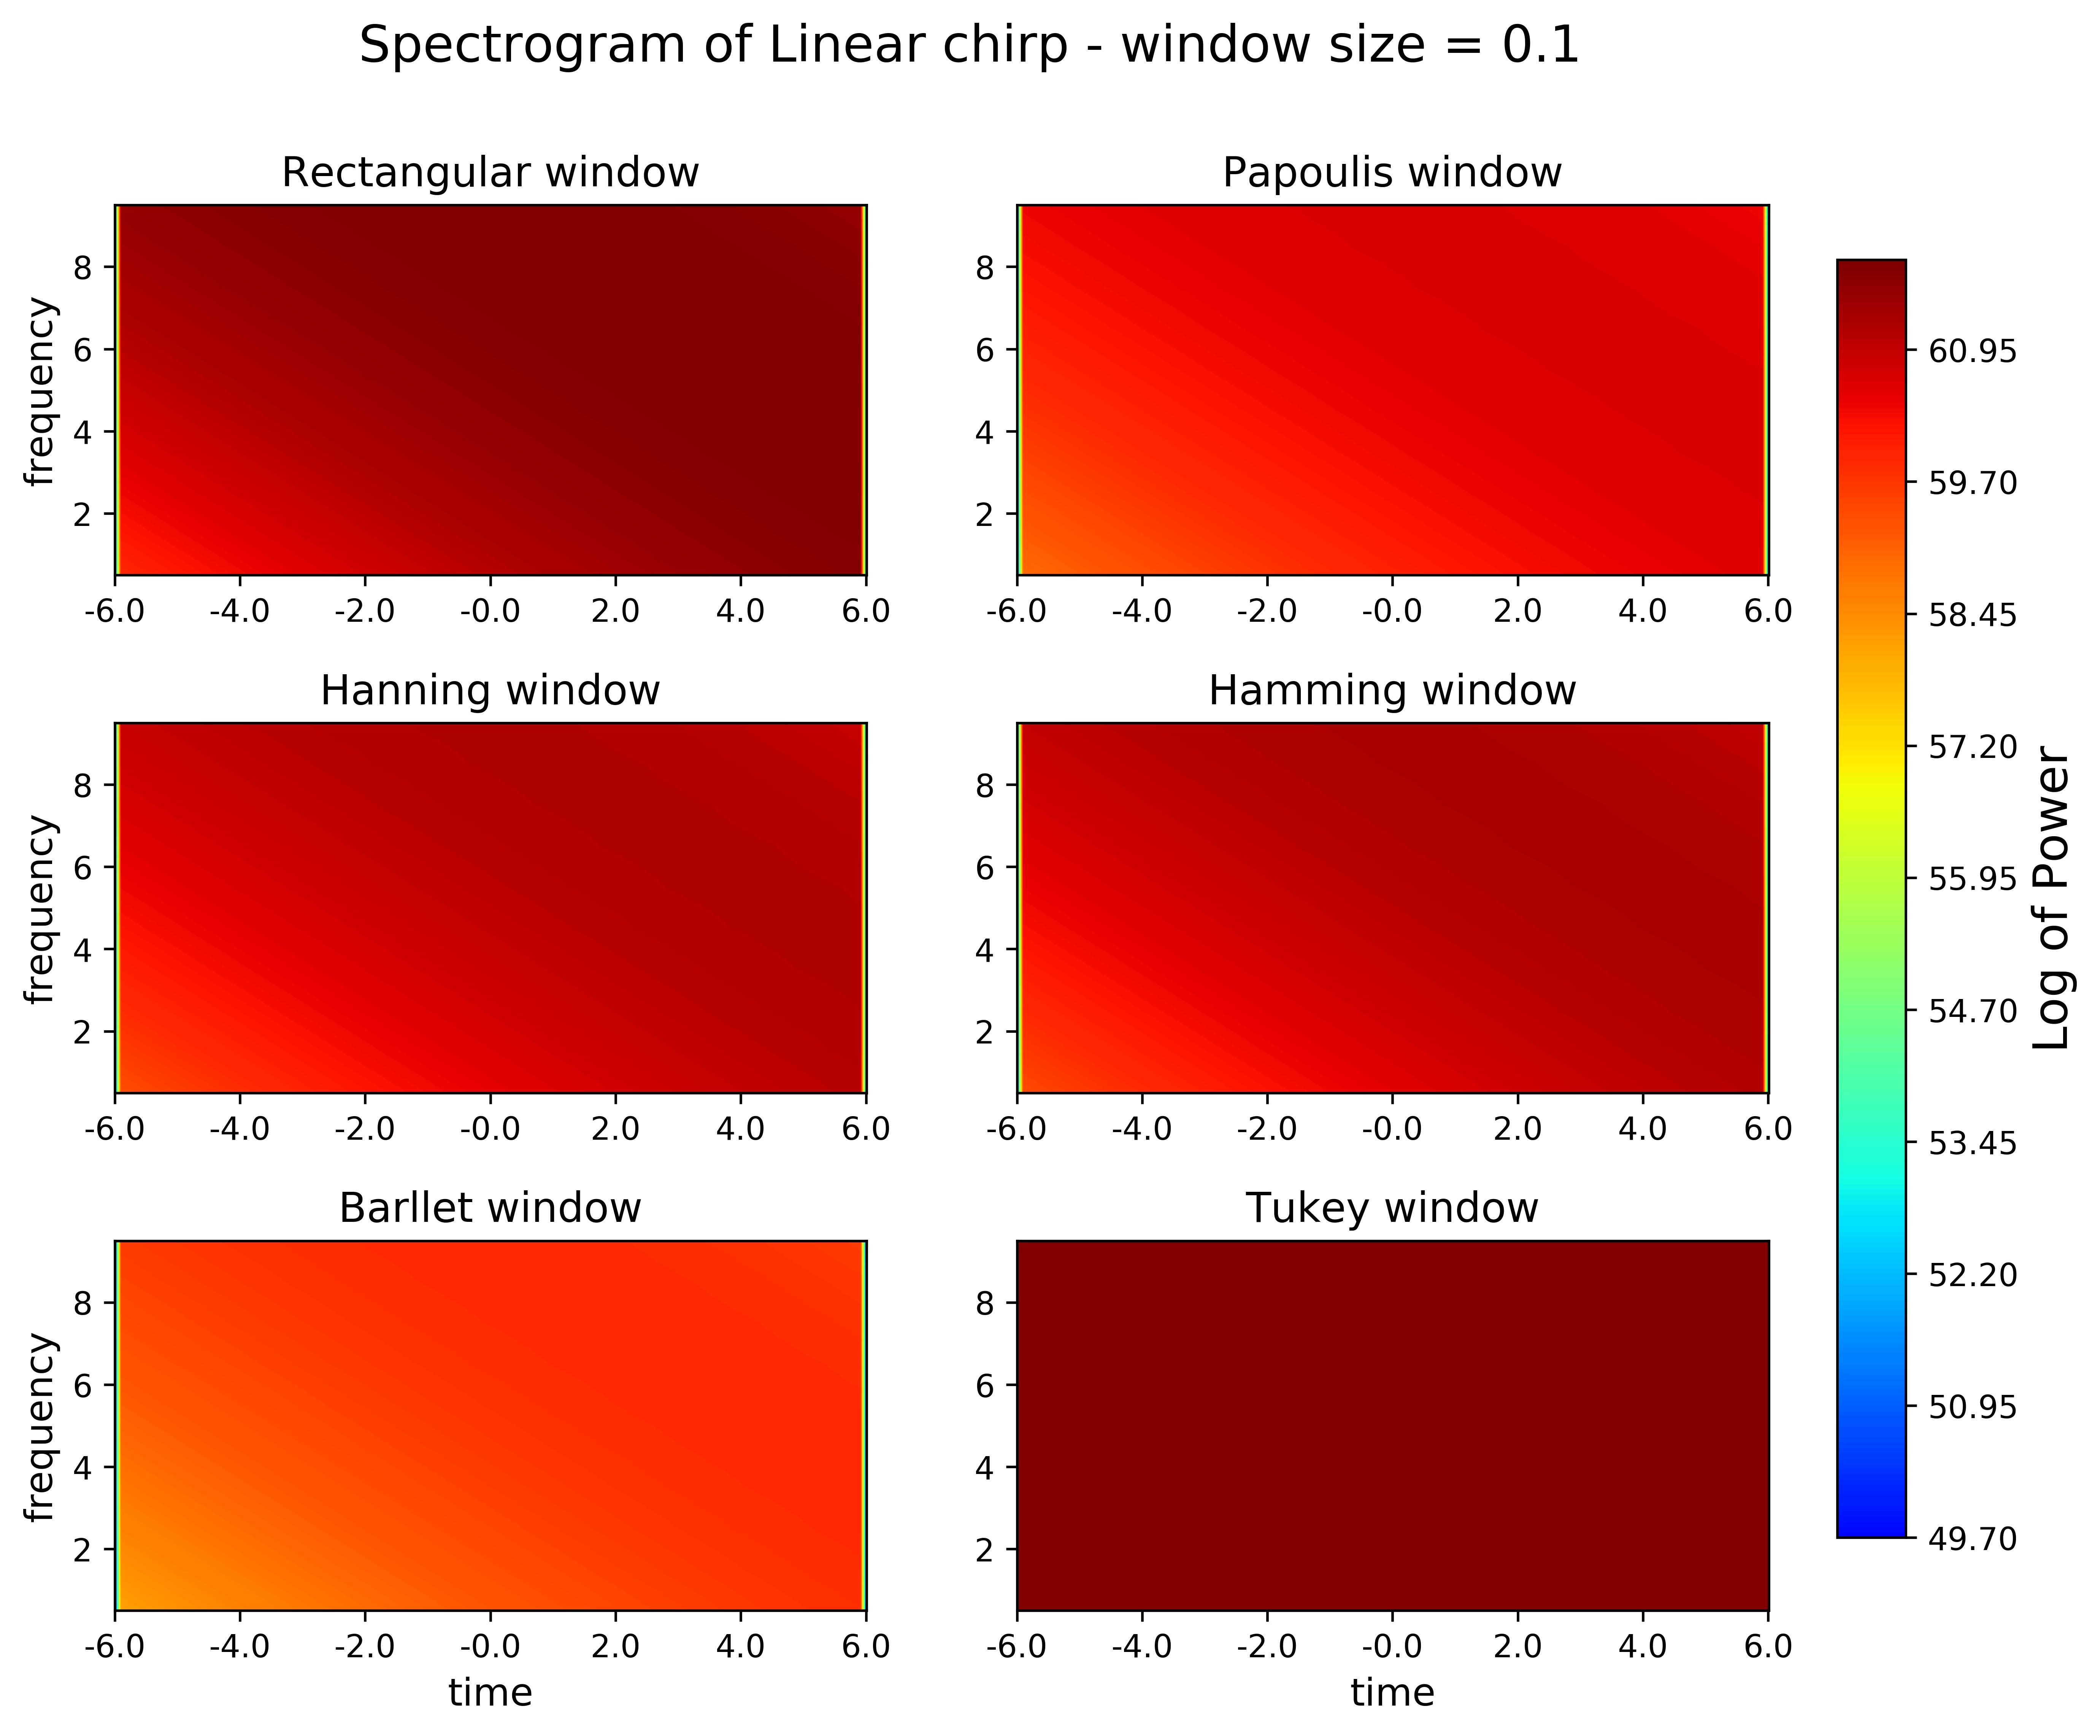
\includegraphics{../scripts/exercicio2/espectros/Linear_ws0.1.jpg}}	
	\end{center}
	\vspace{1mm}
	\label{ex1_fig1}
\end{figure}

Espectrogramas do \textbf{chirp linear}, $-6 \leq t \leq 6$ e tamanho das janelas = 0.5: Figura 2.8.

% FIGURA
\begin{figure}[ht!]
	\legenda{Figura 2.8: Espectrogramas do chirp linear com janelas de tamanho igual a 0.5. Comparar com segunda linha (de cima para baixo) da Figura 1.1.}
	\vspace{3mm}	
	\begin{center}
		\resizebox{\textwidth}{!}{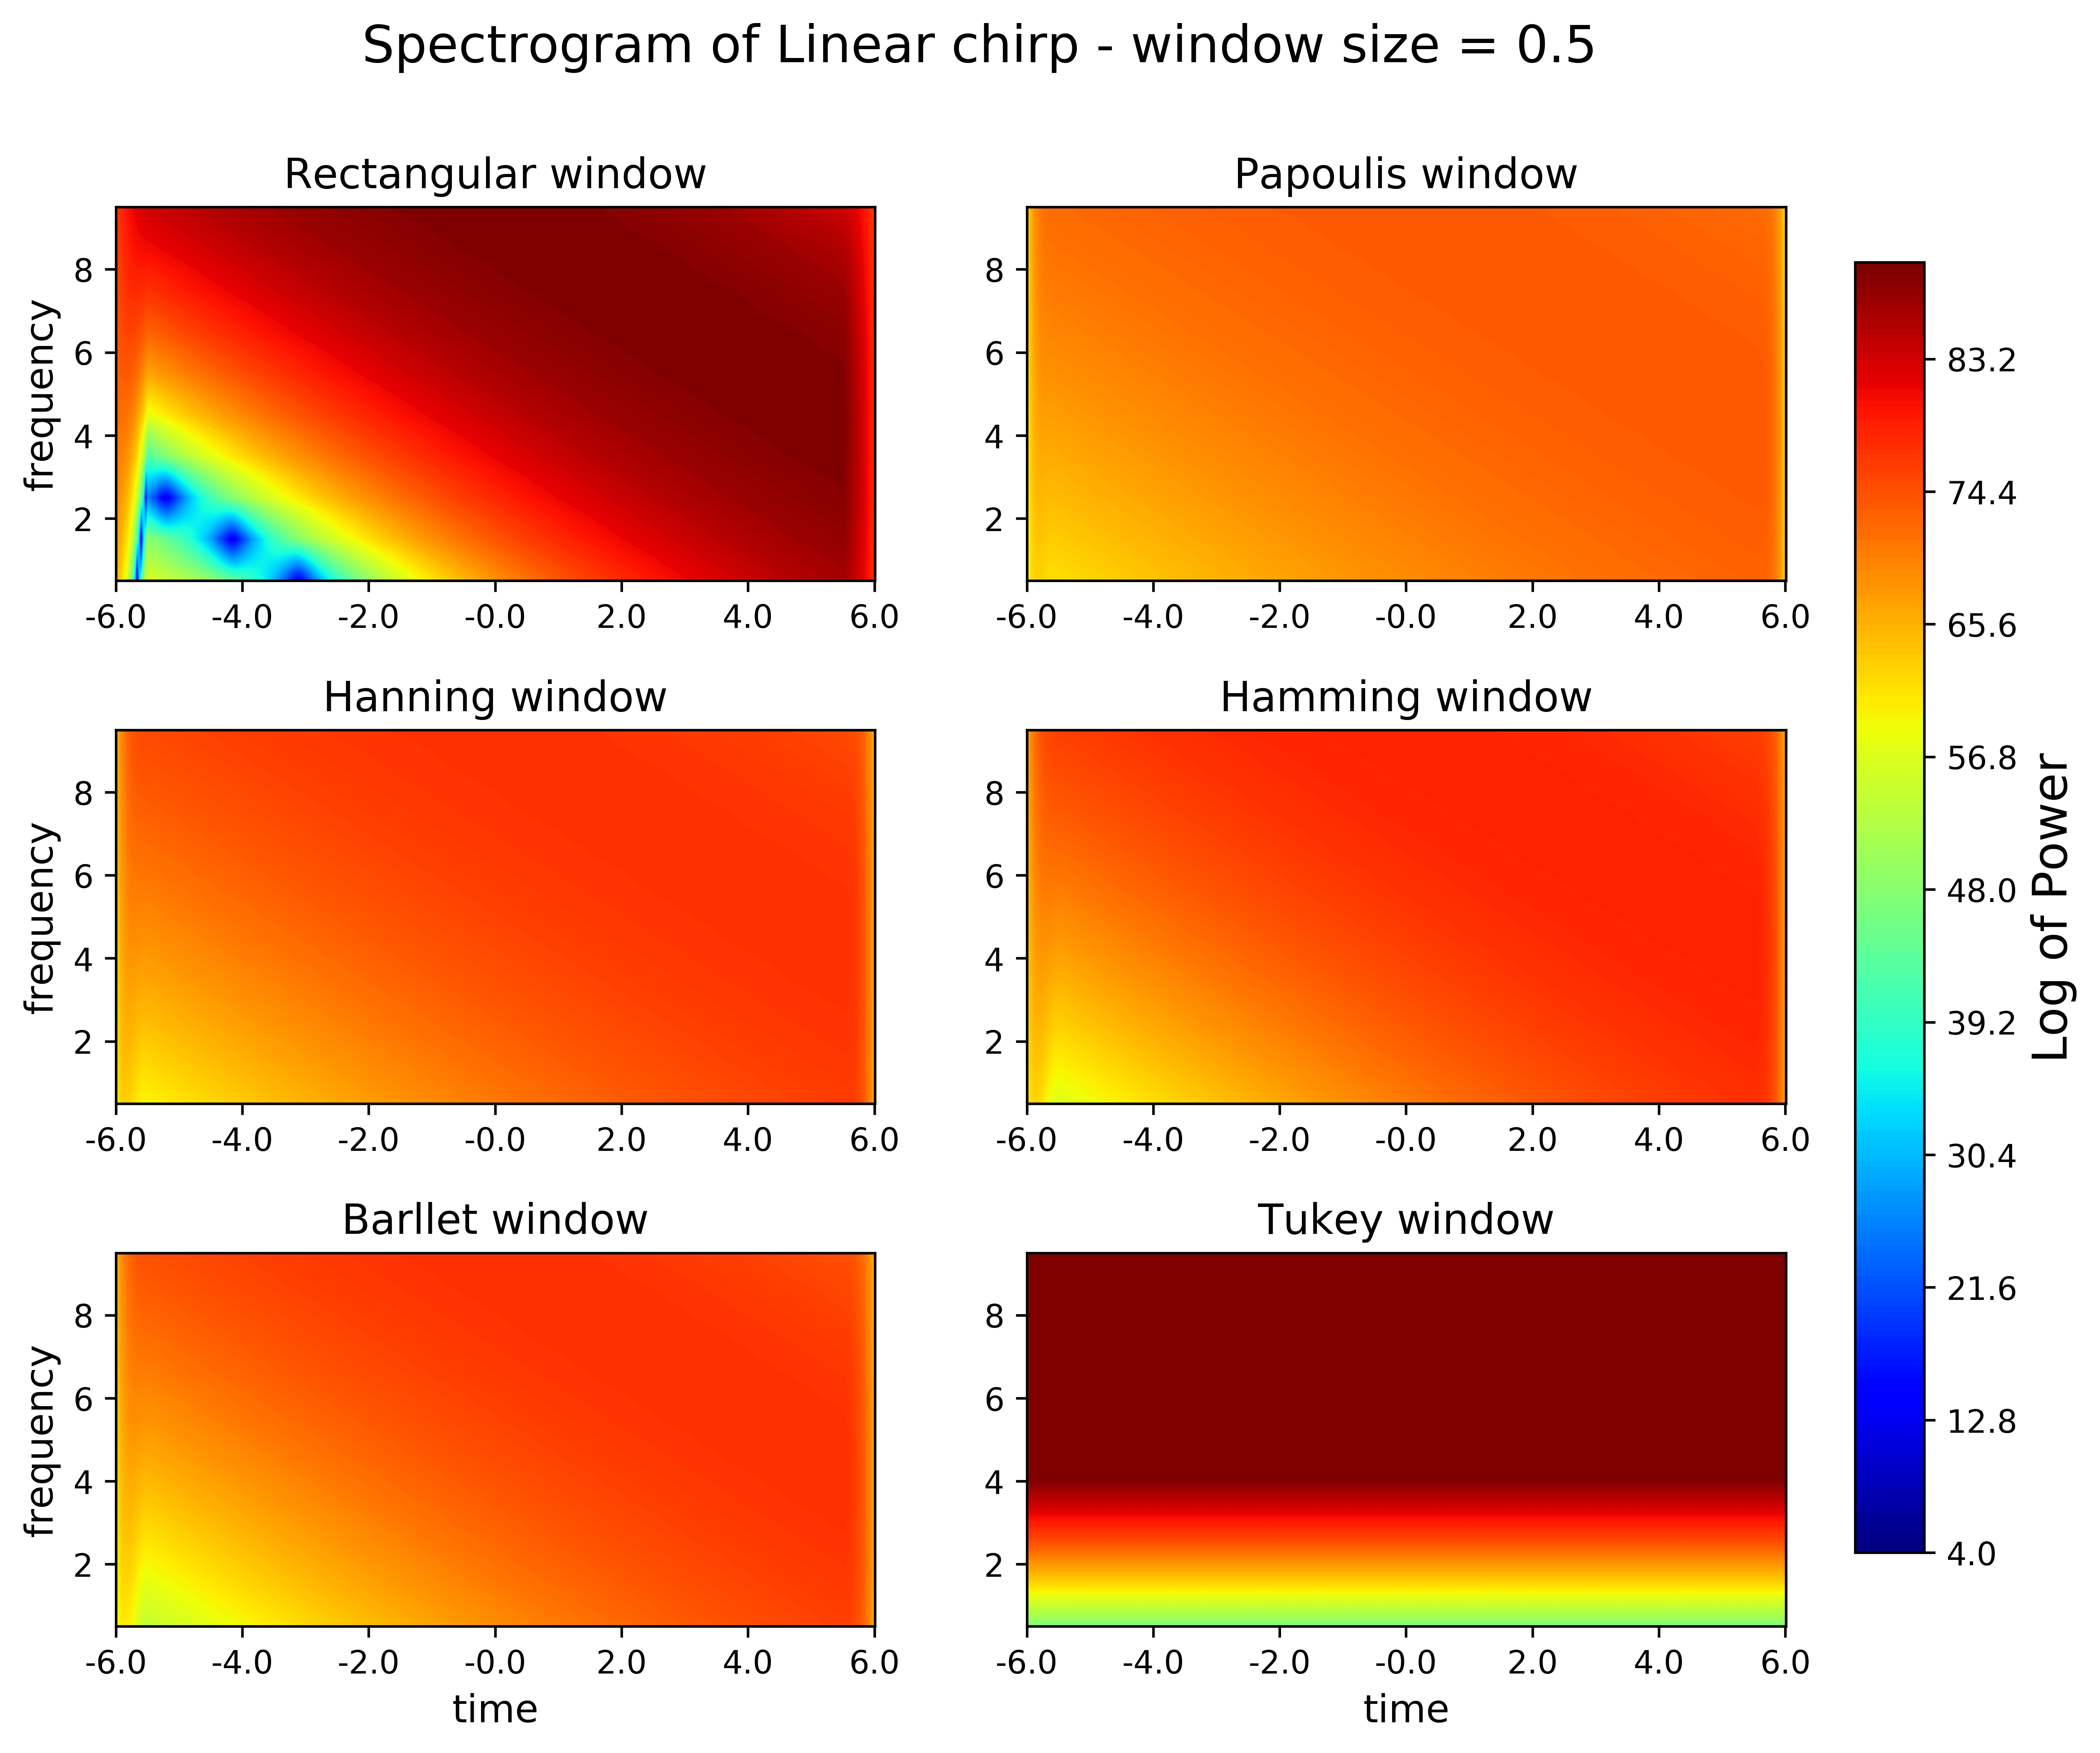
\includegraphics{../scripts/exercicio2/espectros/Linear_ws0.5.jpg}}	
	\end{center}
	\vspace{1mm}
	\label{ex1_fig1}
\end{figure}


Espectrogramas do \textbf{chirp linear}, $0 \leq t \leq 6$ e tamanho das janelas = 0.5: Figura 2.9.

% FIGURA
\begin{figure}[ht!]
	\legenda{Figura 2.9: Espectrogramas do chirp linear com janelas de tamanho igual a 0.5. Comparar com segunda linha (de cima para baixo) da Figura 1.3.}
	\vspace{3mm}	
	\begin{center}
		\resizebox{\textwidth}{!}{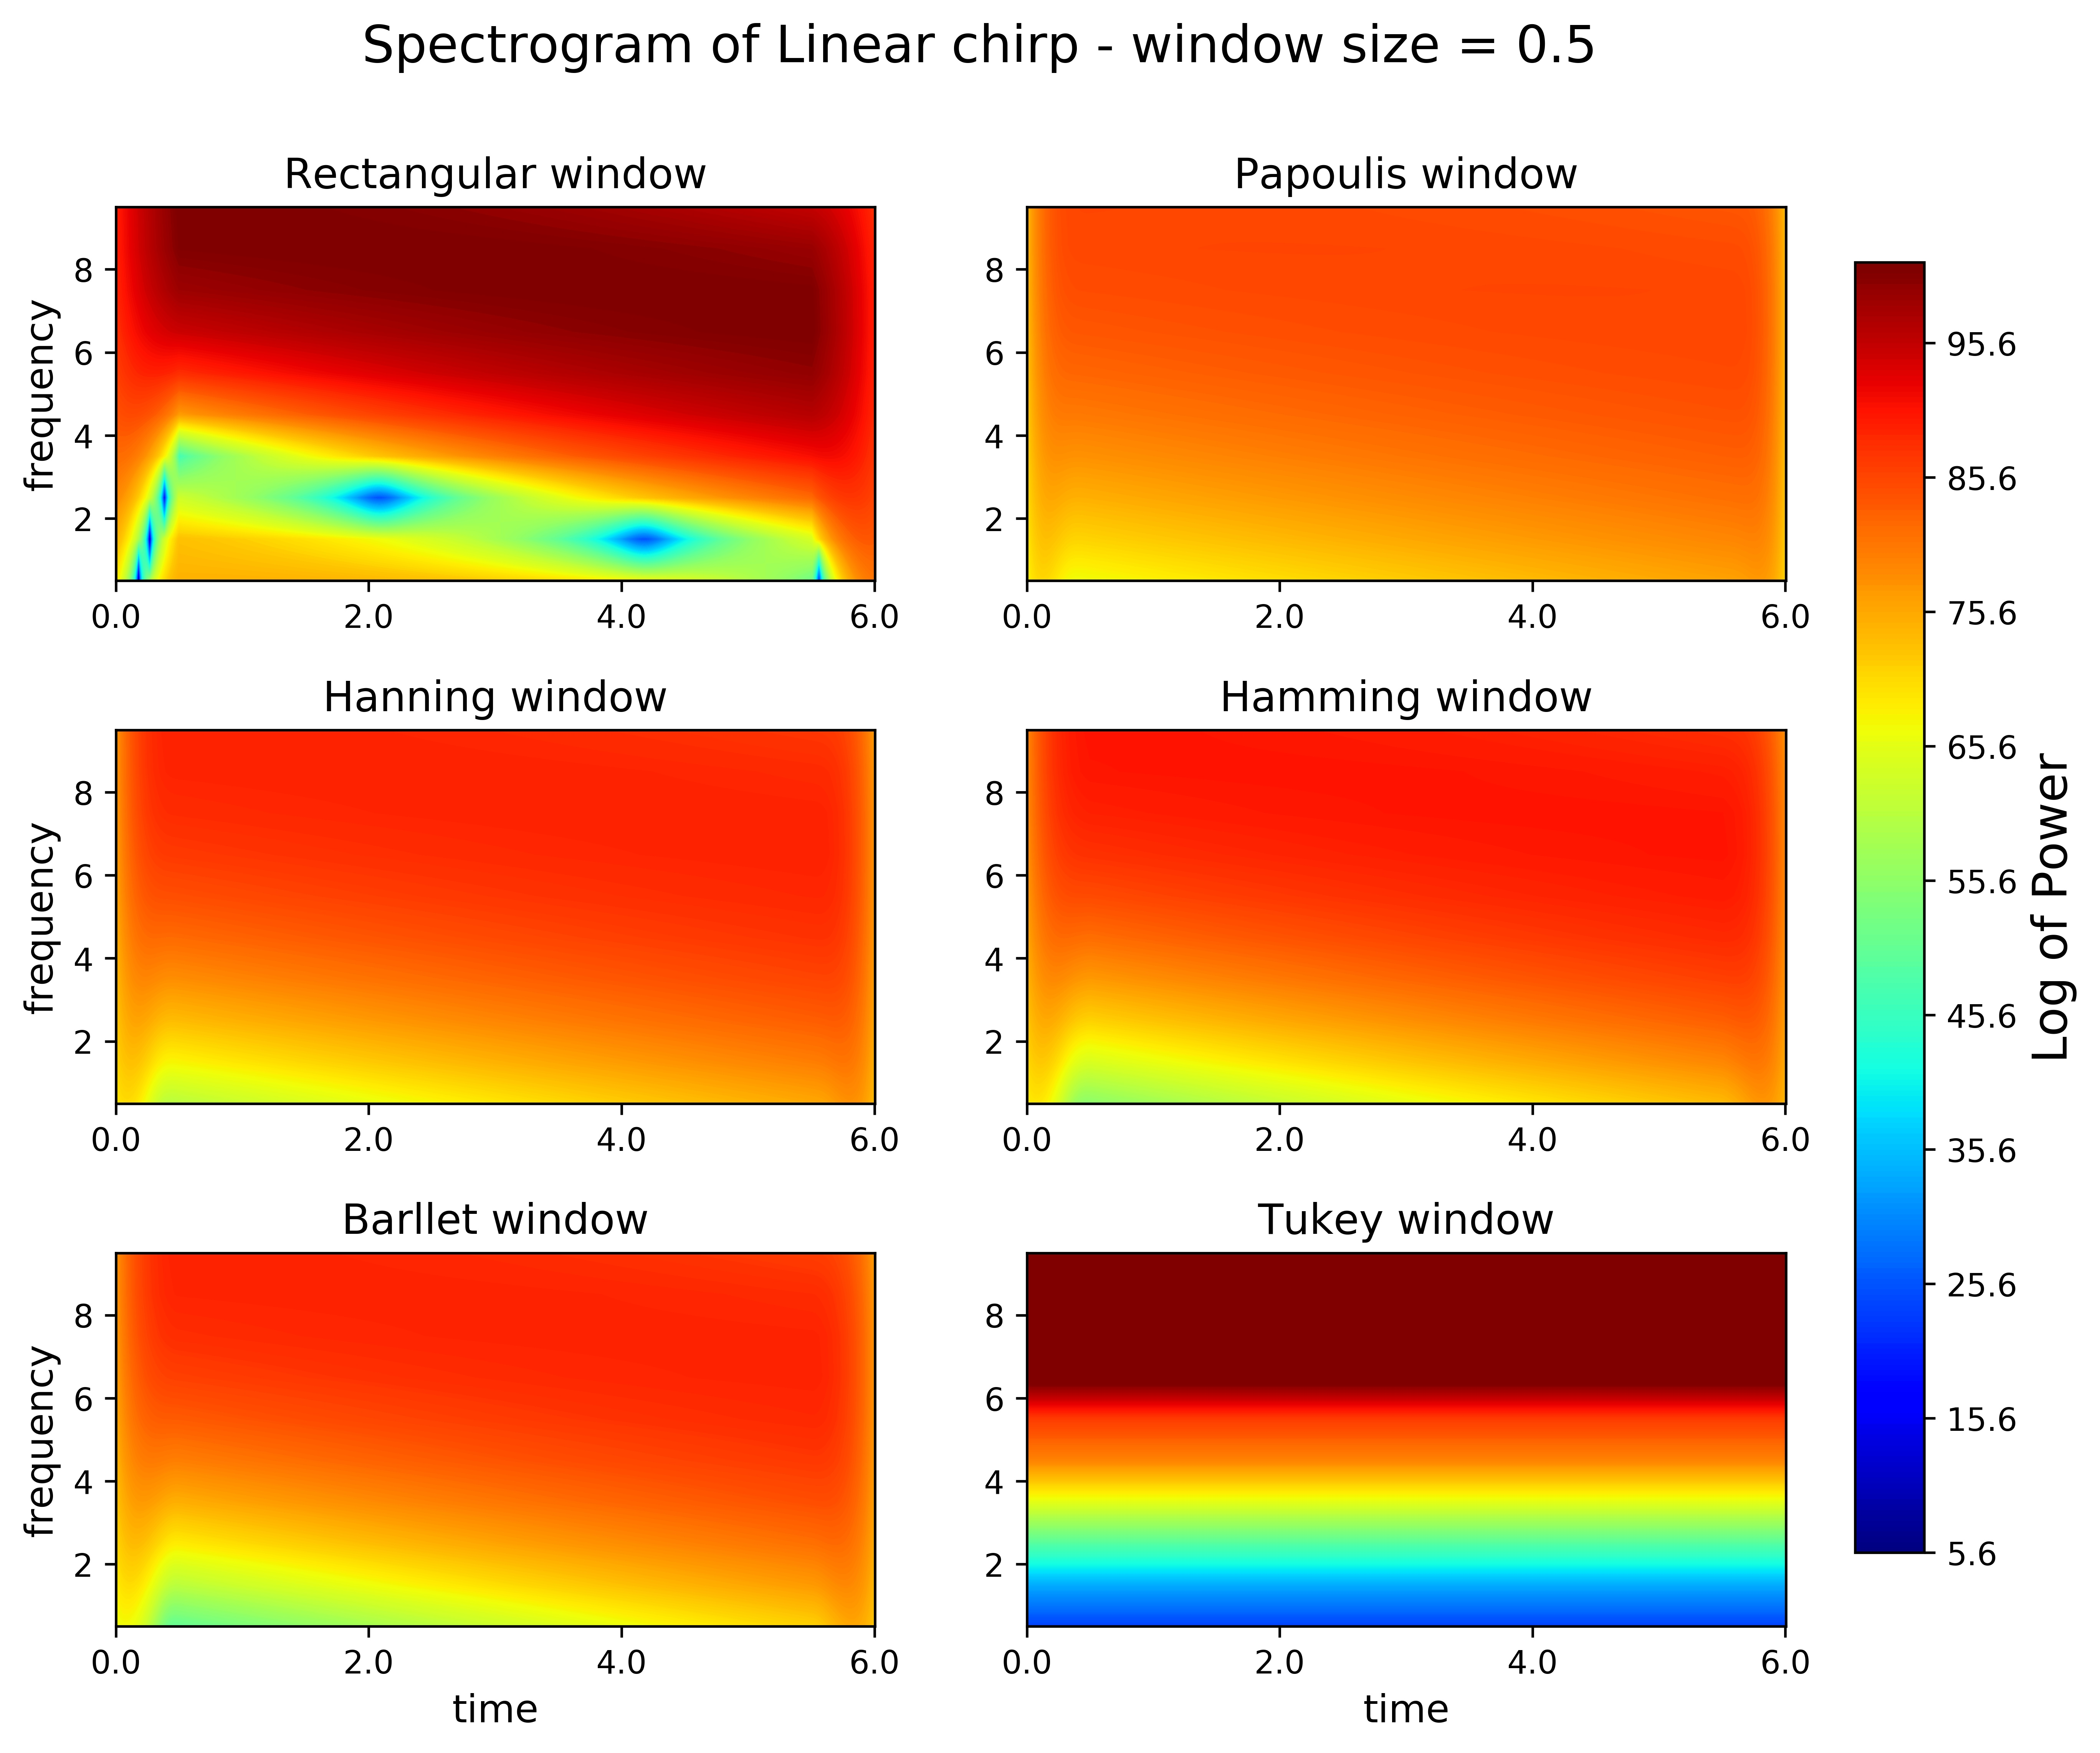
\includegraphics{../scripts/exercicio2/espectros/TEST_Linear_ws0.5.jpg}}	
	\end{center}
	\vspace{1mm}
	\label{ex1_fig1}
\end{figure}

%%%%%%%%%%%%%%%% Quadratic


Espectrogramas do \textbf{chirp quadrático}, $-4 \leq t \leq 4$ e tamanho das janelas = 0.1: Figura 2.10.

% FIGURA
\begin{figure}[ht!]
	\legenda{Figura 2.10: Espectrogramas do chirp quadrático com janelas de tamanho igual a 0.1. Comparar com terceira linha (de cima para baixo) da Figura 1.1.}
	\vspace{3mm}	
	\begin{center}
		\resizebox{\textwidth}{!}{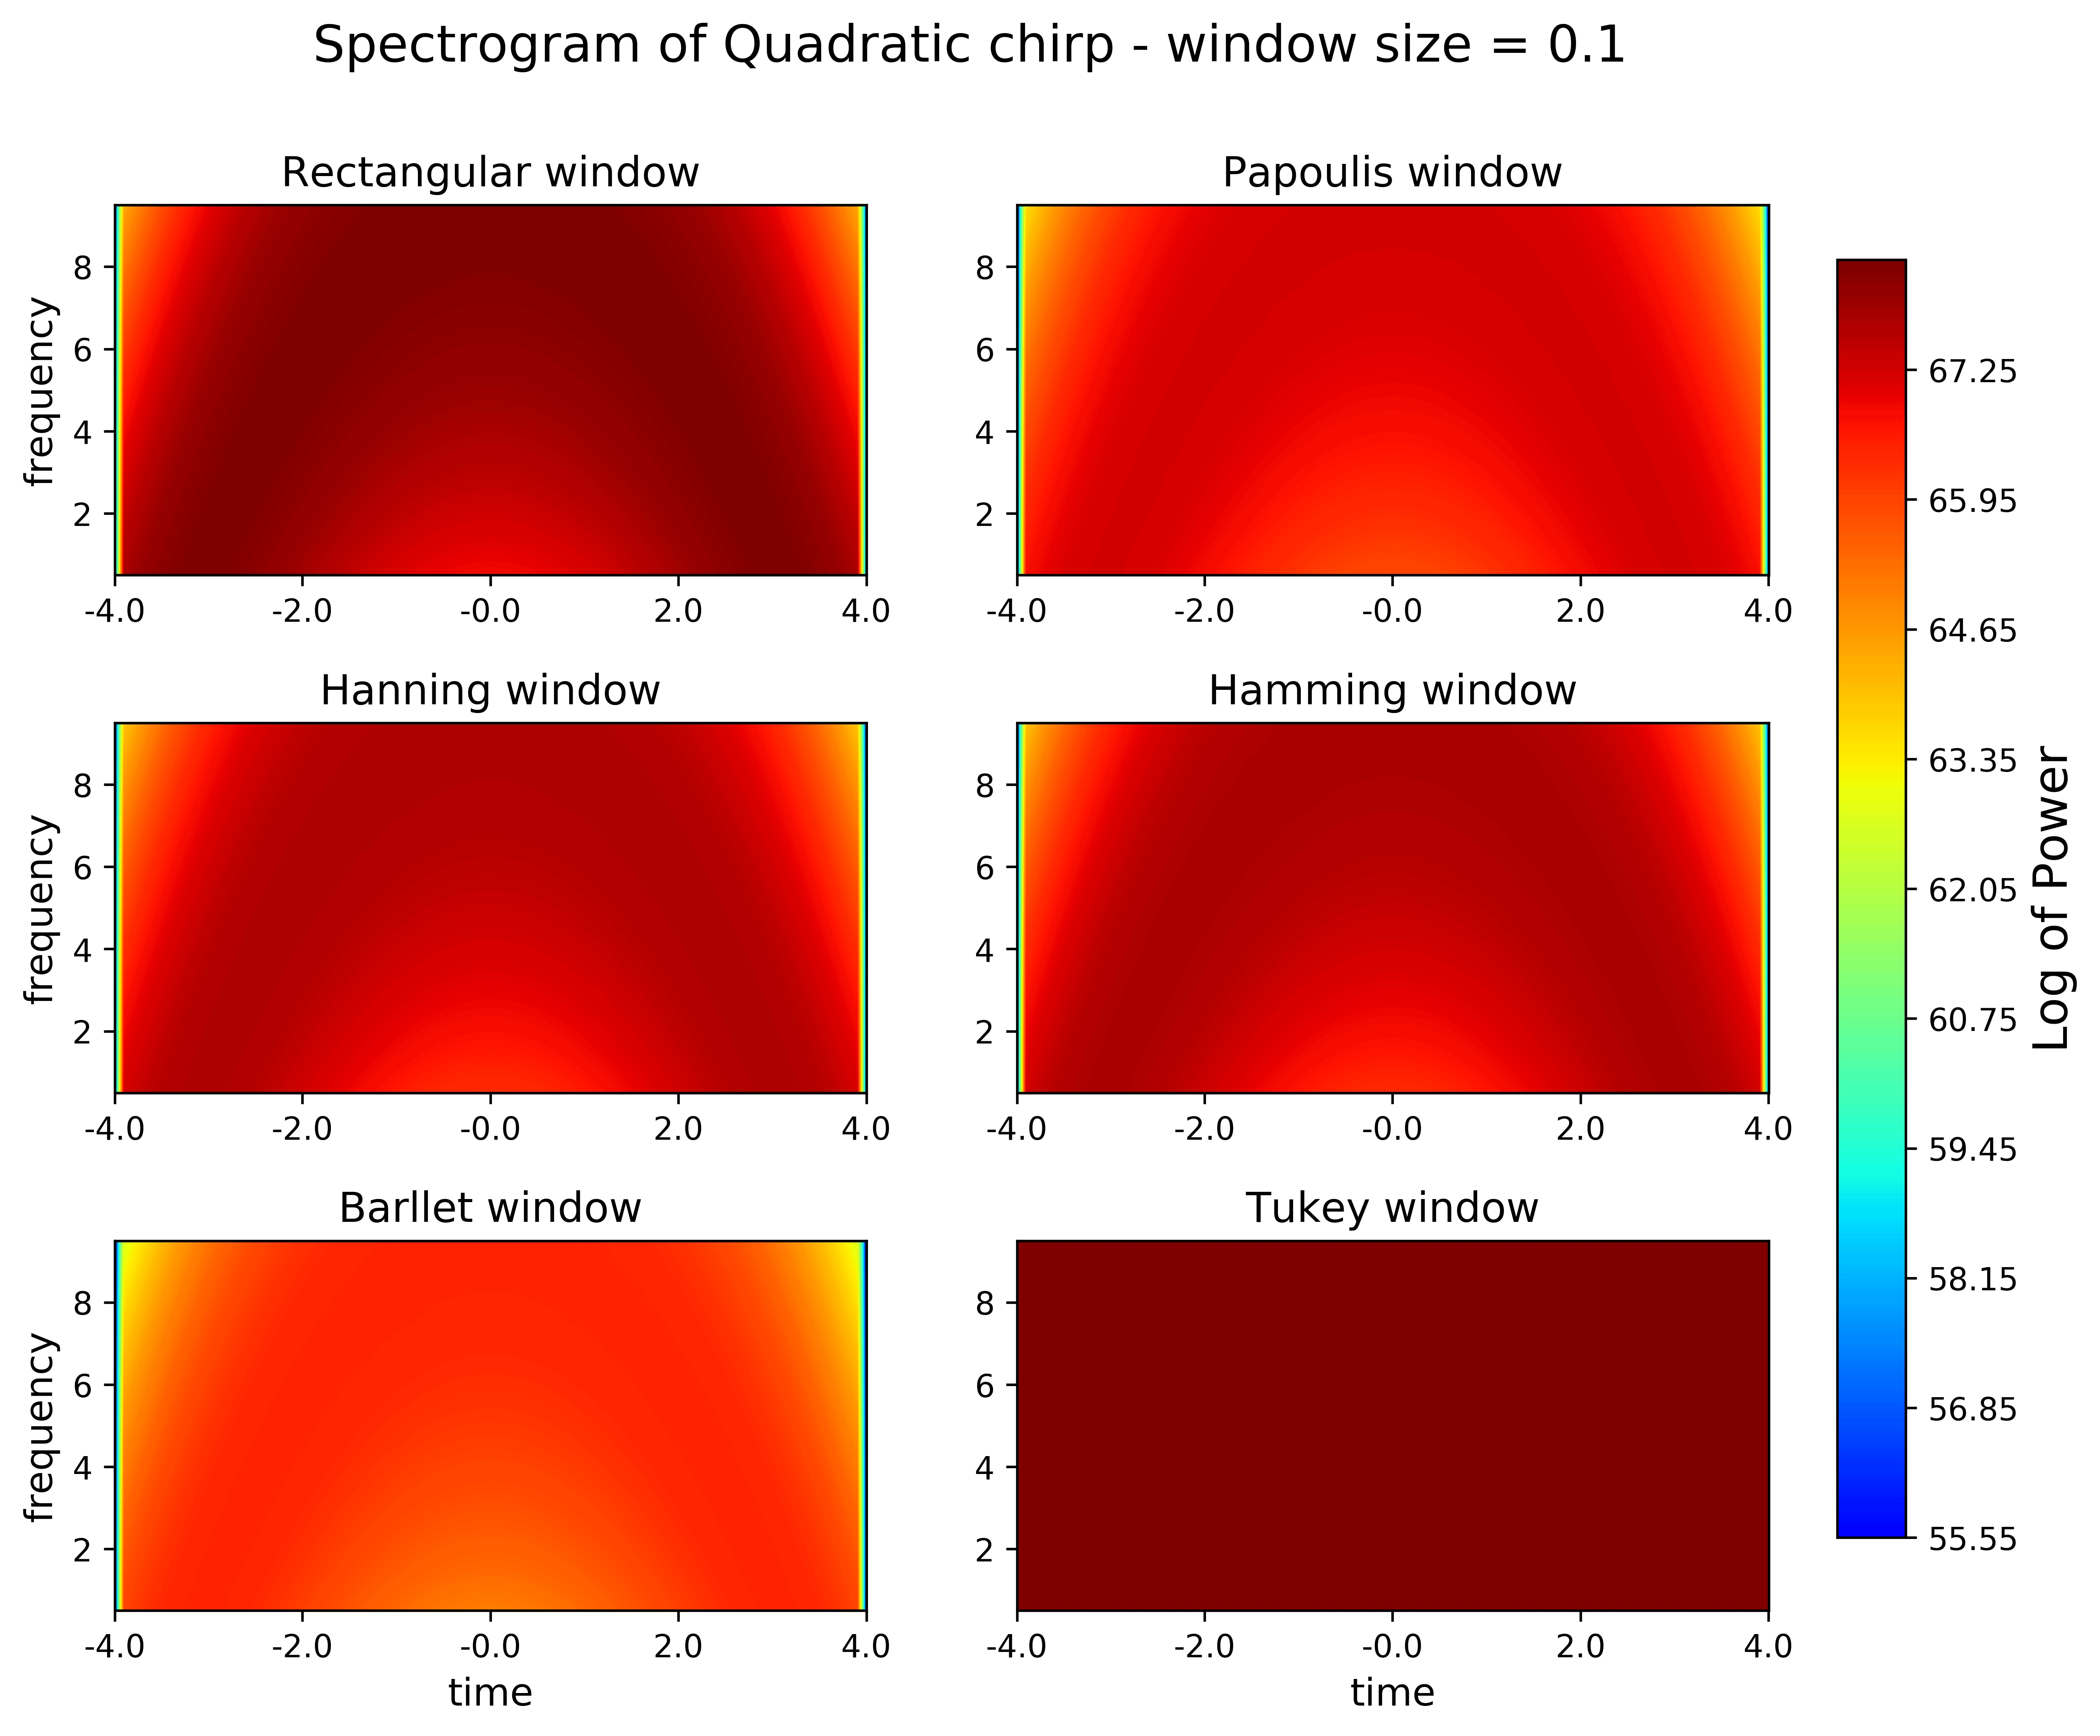
\includegraphics{../scripts/exercicio2/espectros/Quadratic_ws0.1.jpg}}	
	\end{center}
	\vspace{1mm}
	\label{ex1_fig1}
\end{figure}

Espectrogramas do \textbf{chirp quadrático}, $-4 \leq t \leq 4$ e tamanho das janelas = 0.5: Figura 2.11.

% FIGURA
\begin{figure}[ht!]
	\legenda{Figura 2.11: Espectrogramas do chirp quadrático com janelas de tamanho igual a 0.5. Comparar com terceira linha (de cima para baixo) da Figura 1.1.}
	\vspace{3mm}	
	\begin{center}
		\resizebox{\textwidth}{!}{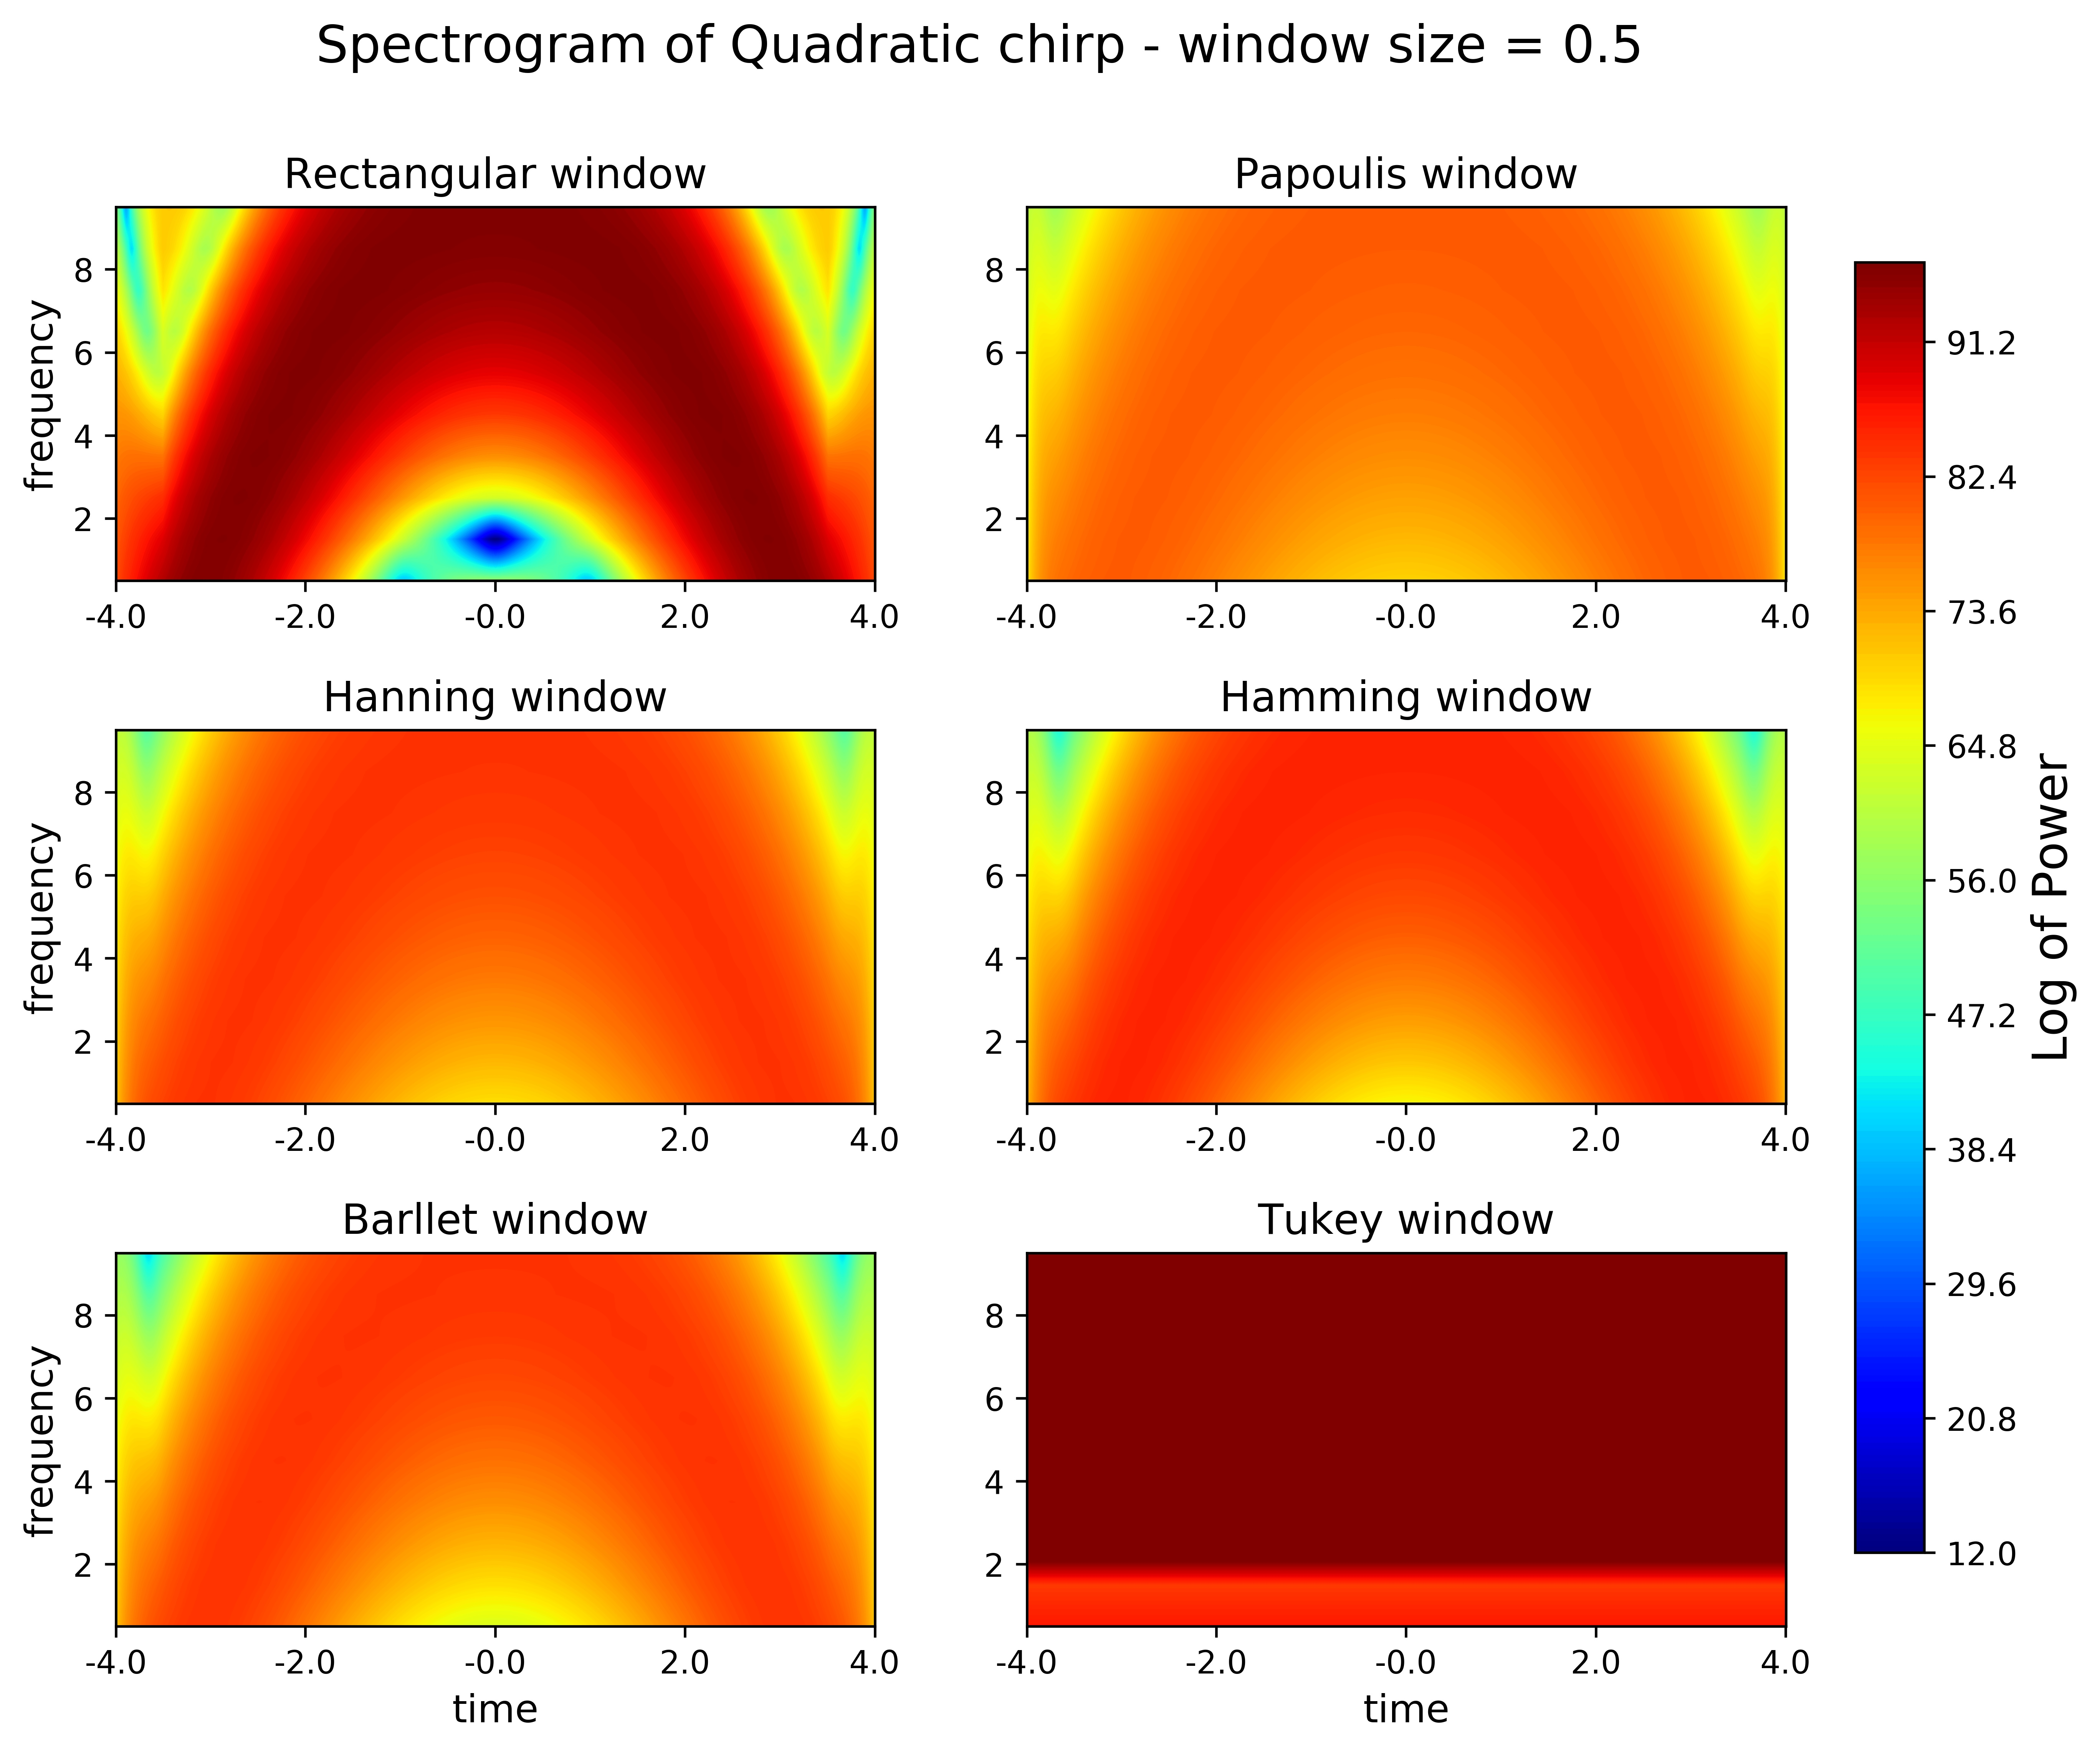
\includegraphics{../scripts/exercicio2/espectros/Quadratic_ws0.5.jpg}}	
	\end{center}
	\vspace{1mm}
	\label{ex1_fig1}
\end{figure}


Espectrogramas do \textbf{chirp quadrático}, $0 \leq t \leq 6$ e tamanho das janelas = 0.5: Figura 2.12.

% FIGURA
\begin{figure}[ht!]
	\legenda{Figura 2.12: Espectrogramas do chirp quadrático com janelas de tamanho igual a 0.5. Comparar com terceira linha (de cima para baixo) da Figura 1.3.}
	\vspace{3mm}	
	\begin{center}
		\resizebox{\textwidth}{!}{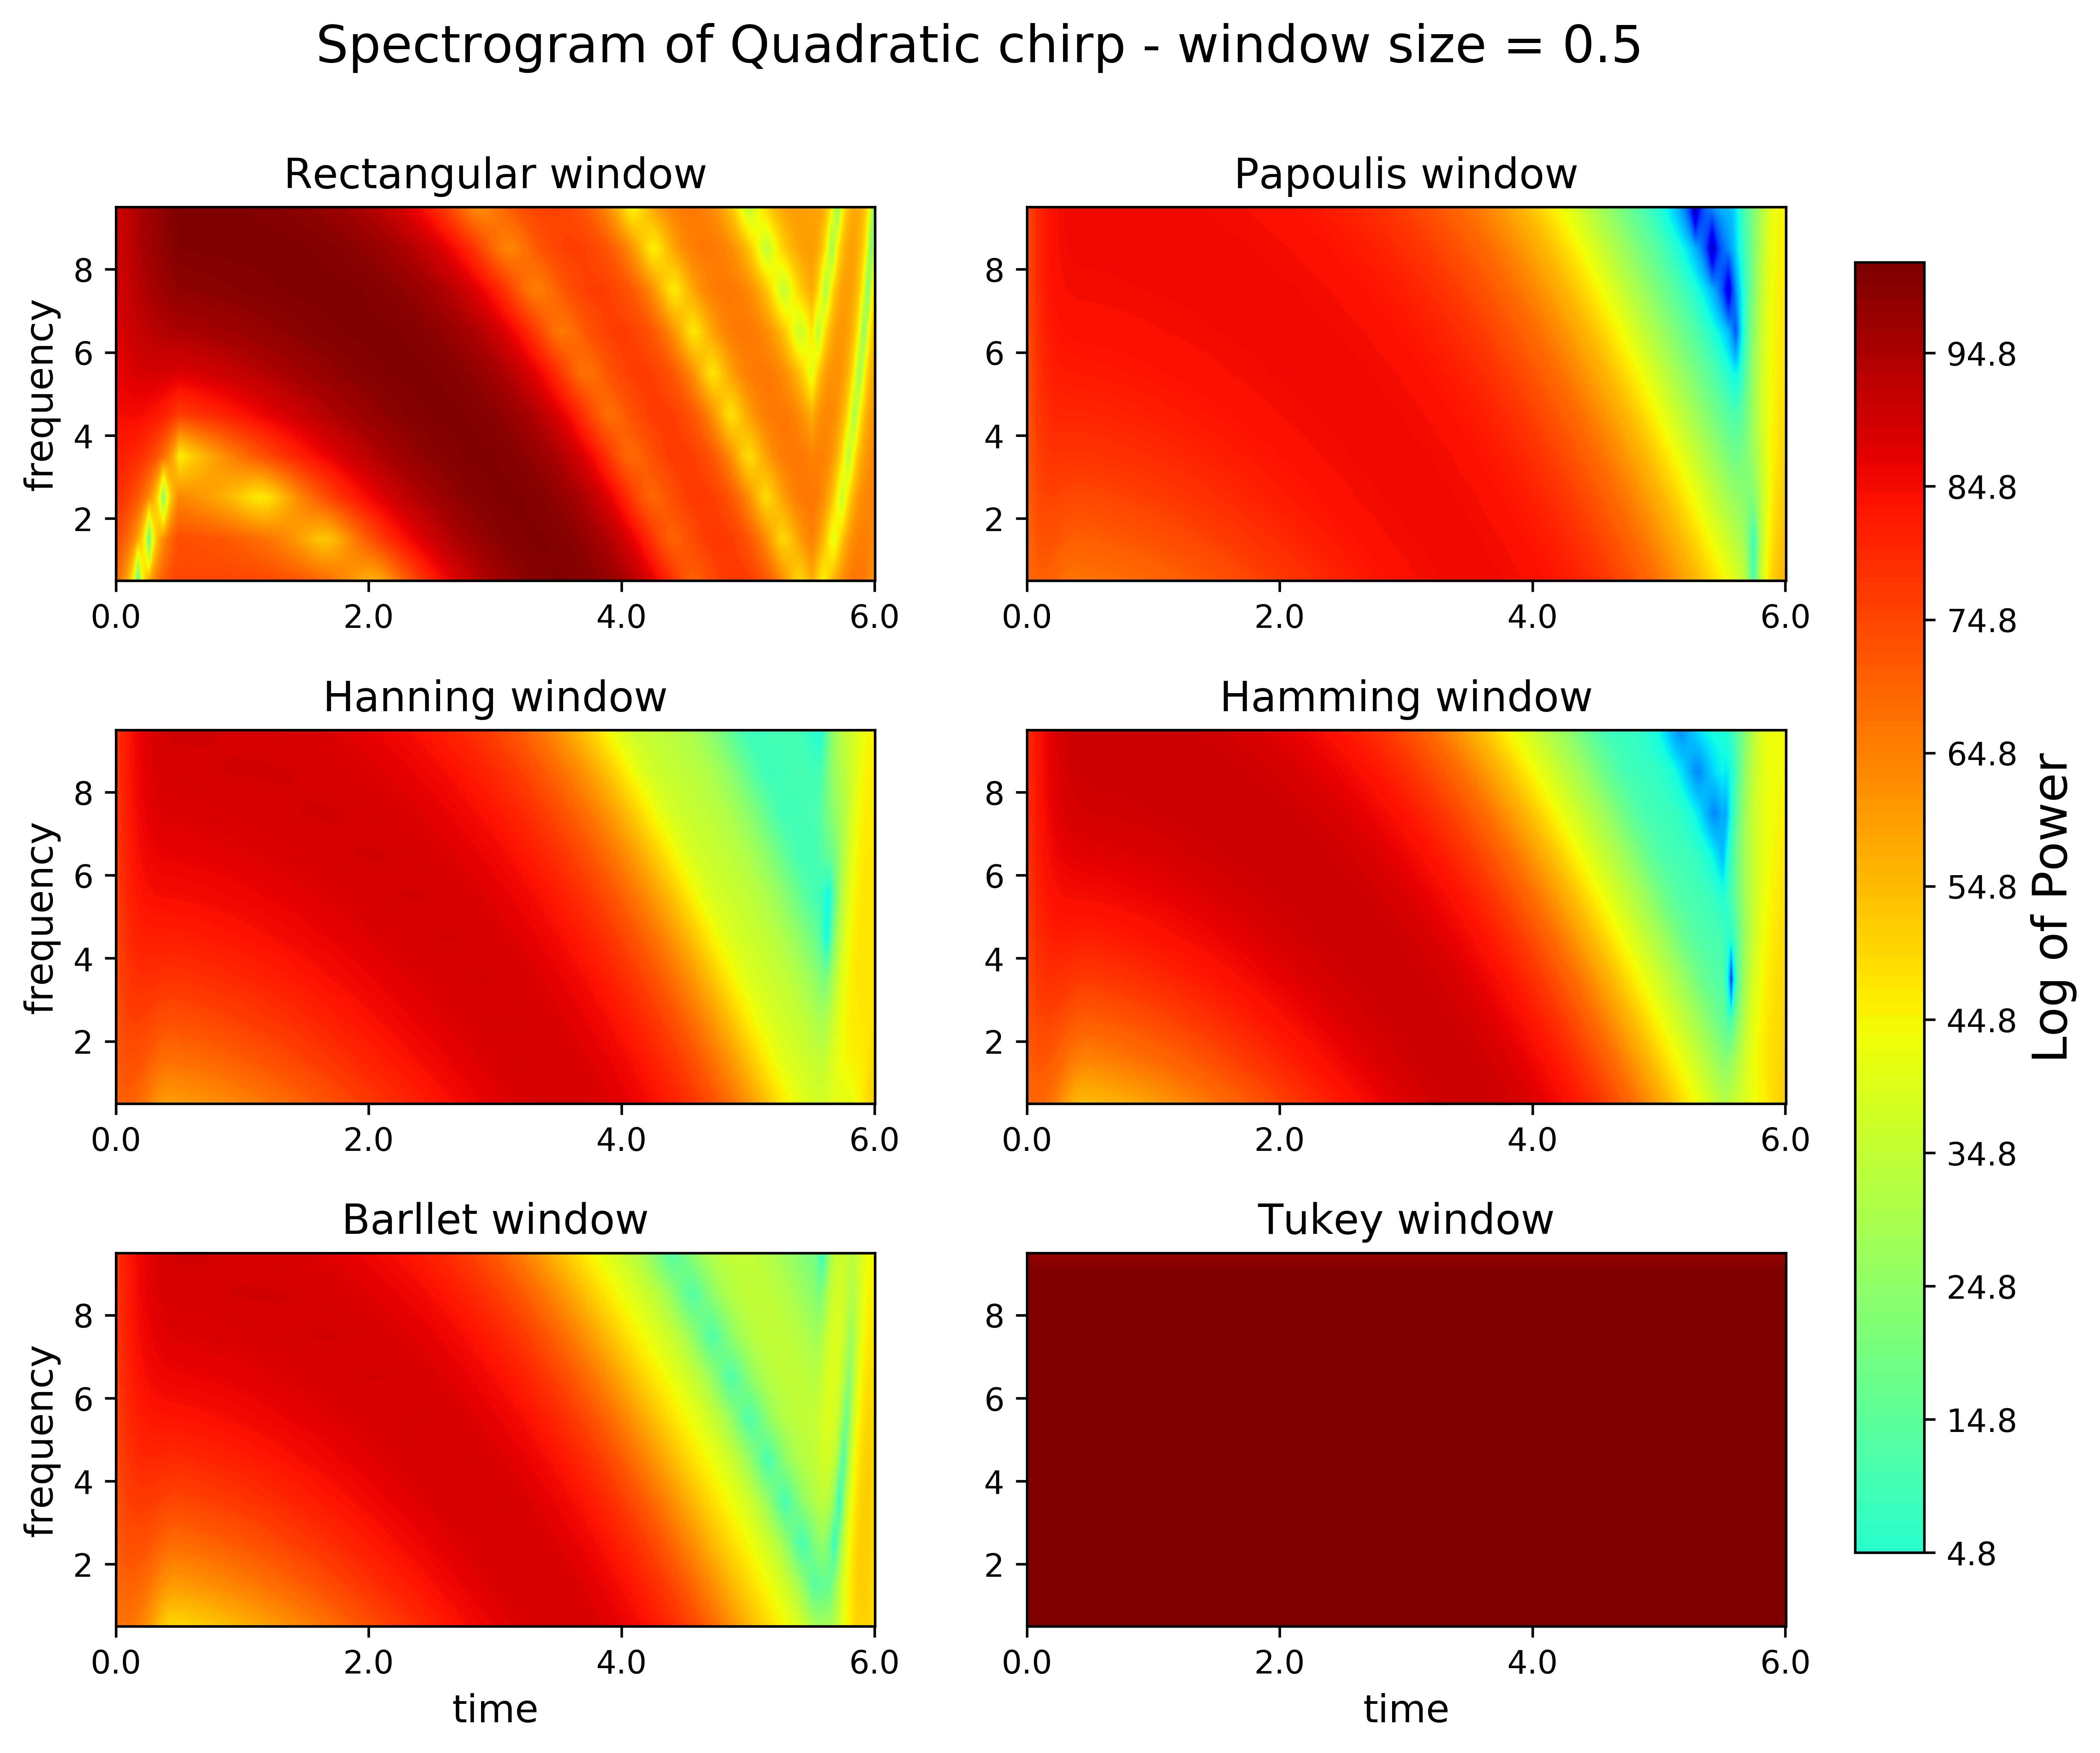
\includegraphics{../scripts/exercicio2/espectros/TEST_Quadratic_ws0.5.jpg}}	
	\end{center}
	\vspace{1mm}
	\label{ex1_fig1}
\end{figure}


%%%%%%%%%%%%%%%% Hyperbolic


Espectrogramas do \textbf{chirp hiperbólico}, $0 \leq t \leq 2$ e tamanho das janelas = 0.1: Figura 2.13.

% FIGURA
\begin{figure}[ht!]
	\legenda{Figura 2.13: Espectrogramas do chirp hiperbólico com janelas de tamanho igual a 0.1. Comparar com última linha da Figura 1.1.}
	\vspace{3mm}	
	\begin{center}
		\resizebox{\textwidth}{!}{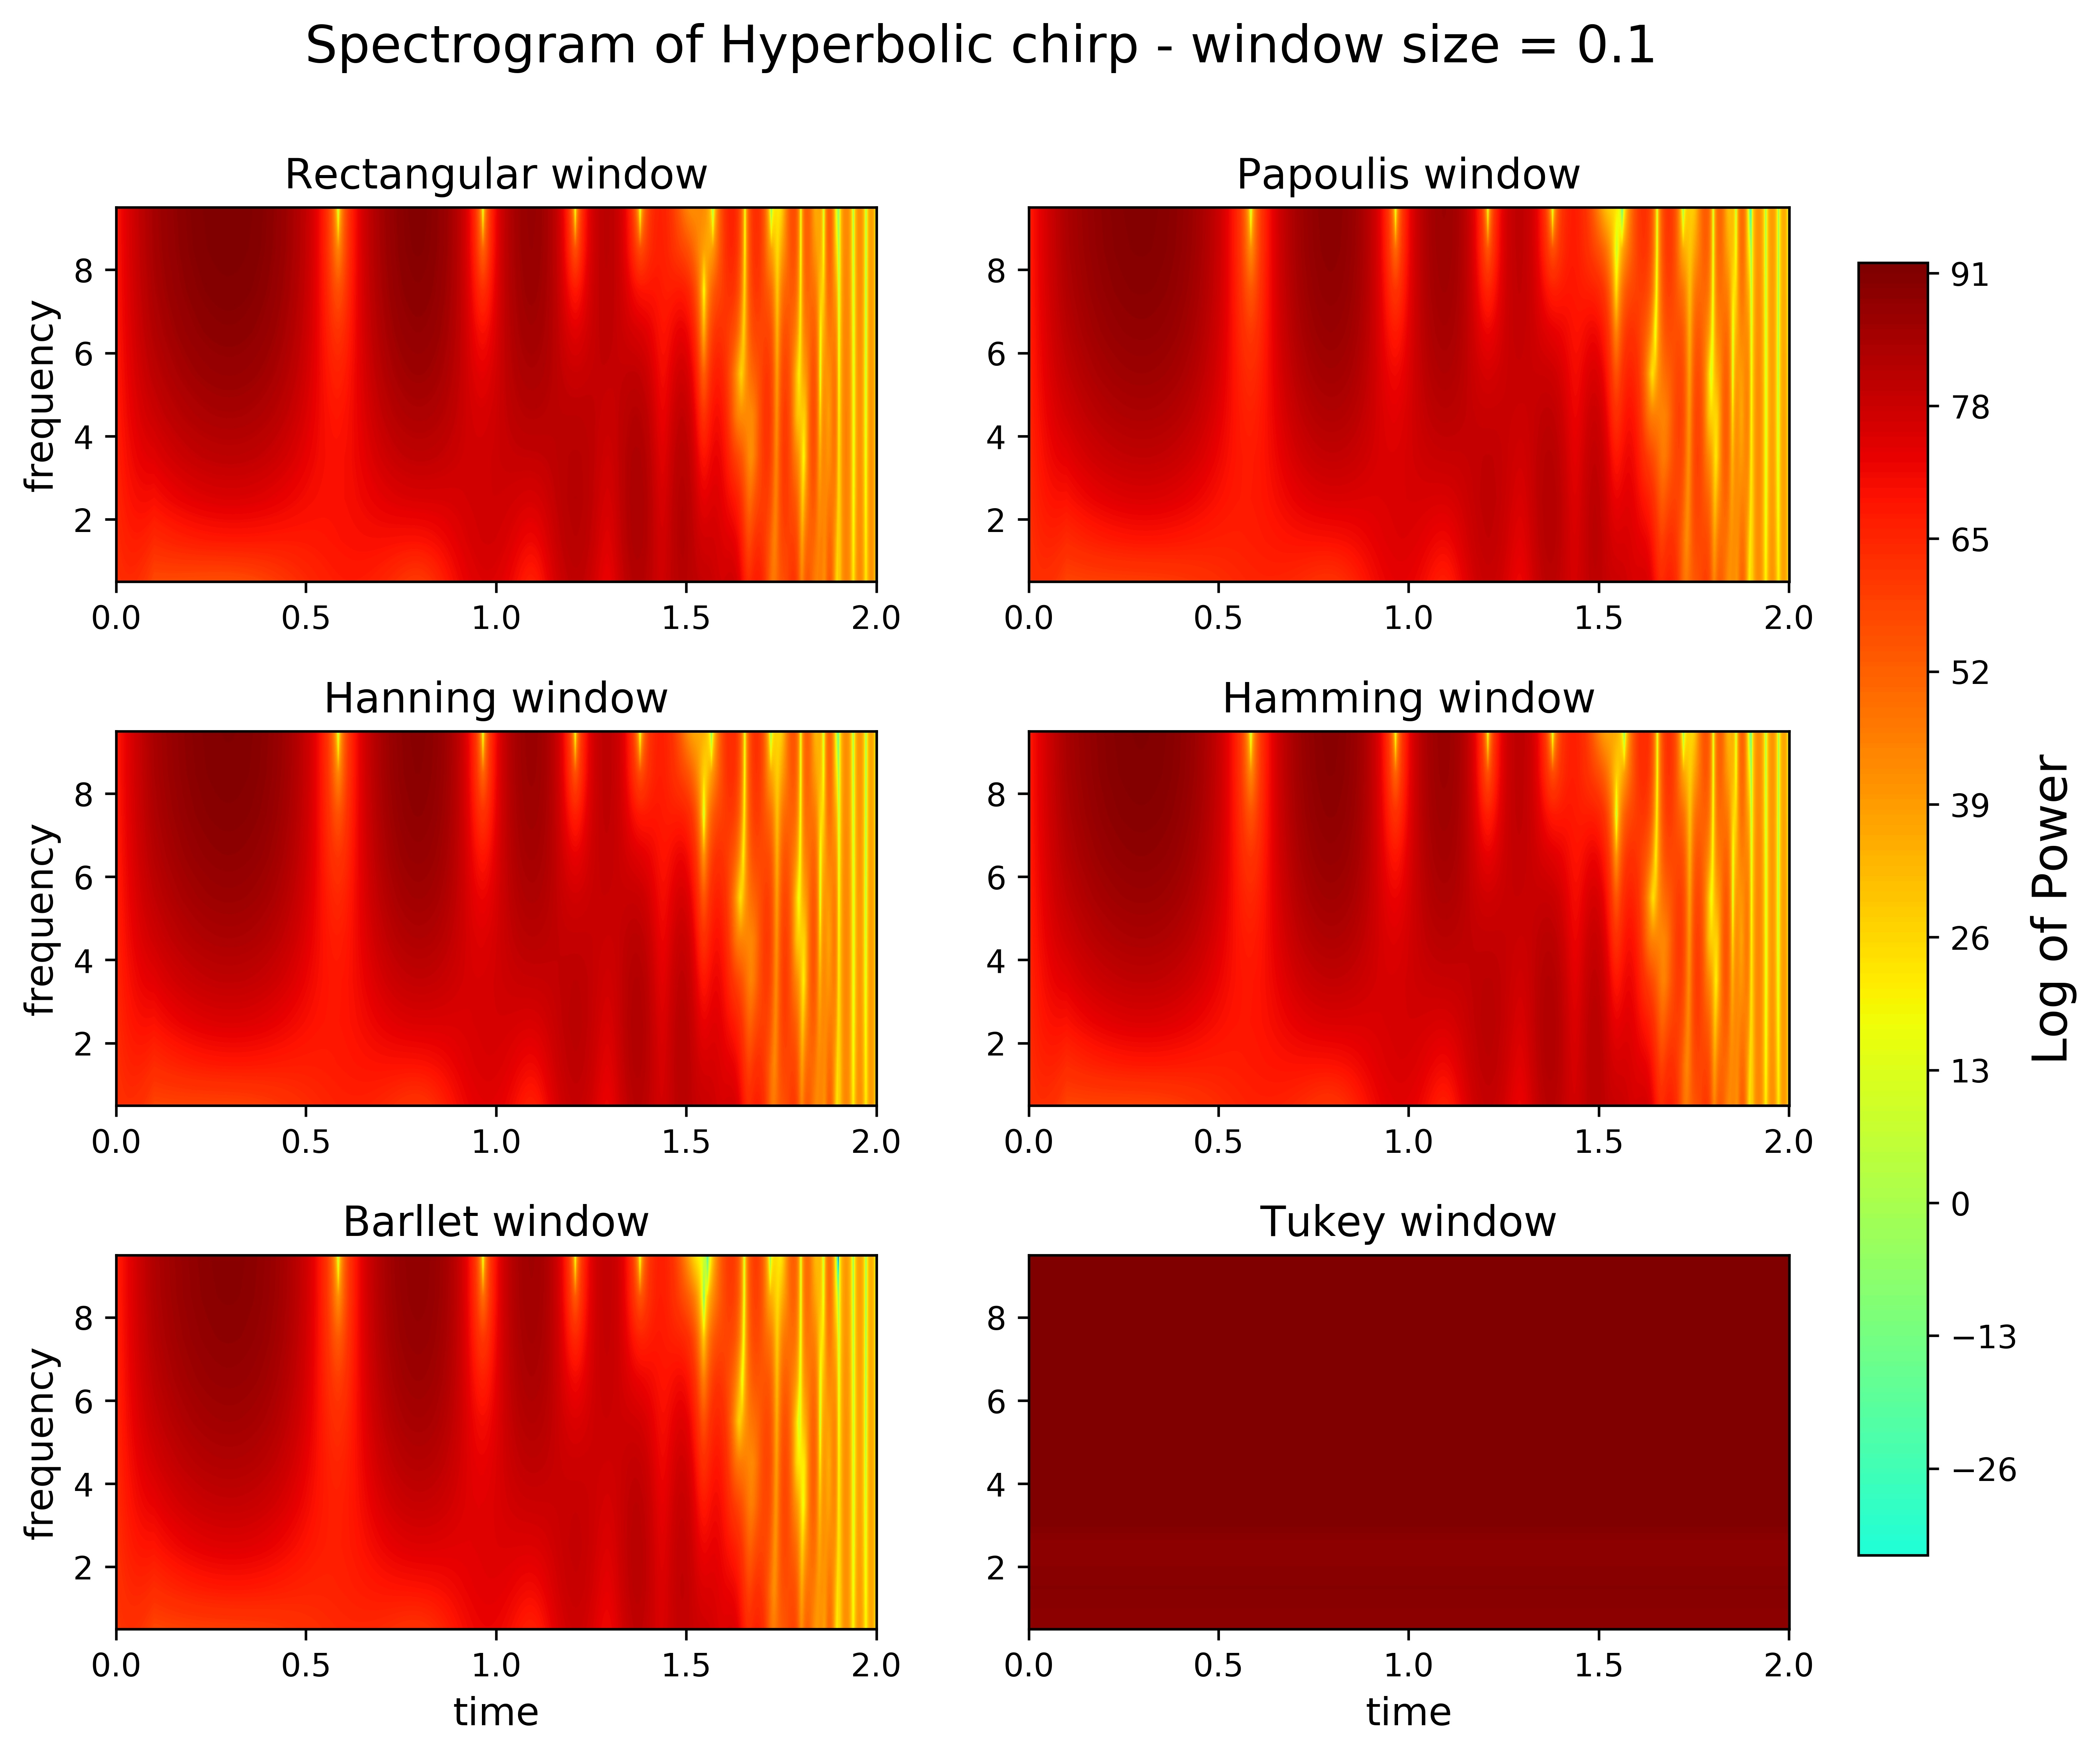
\includegraphics{../scripts/exercicio2/espectros/Hyperbolic_ws0.1.jpg}}	
	\end{center}
	\vspace{1mm}
	\label{ex1_fig1}
\end{figure}

Espectrogramas do \textbf{chirp hiperbólico}, $0 \leq t \leq 2$ e tamanho das janelas = 0.5: Figura 2.14.

% FIGURA
\begin{figure}[ht!]
	\legenda{Figura 2.14: Espectrogramas do chirp hiperbólico com janelas de tamanho igual a 0.5. Comparar com última linha da Figura 1.1.}
	\vspace{3mm}	
	\begin{center}
		\resizebox{\textwidth}{!}{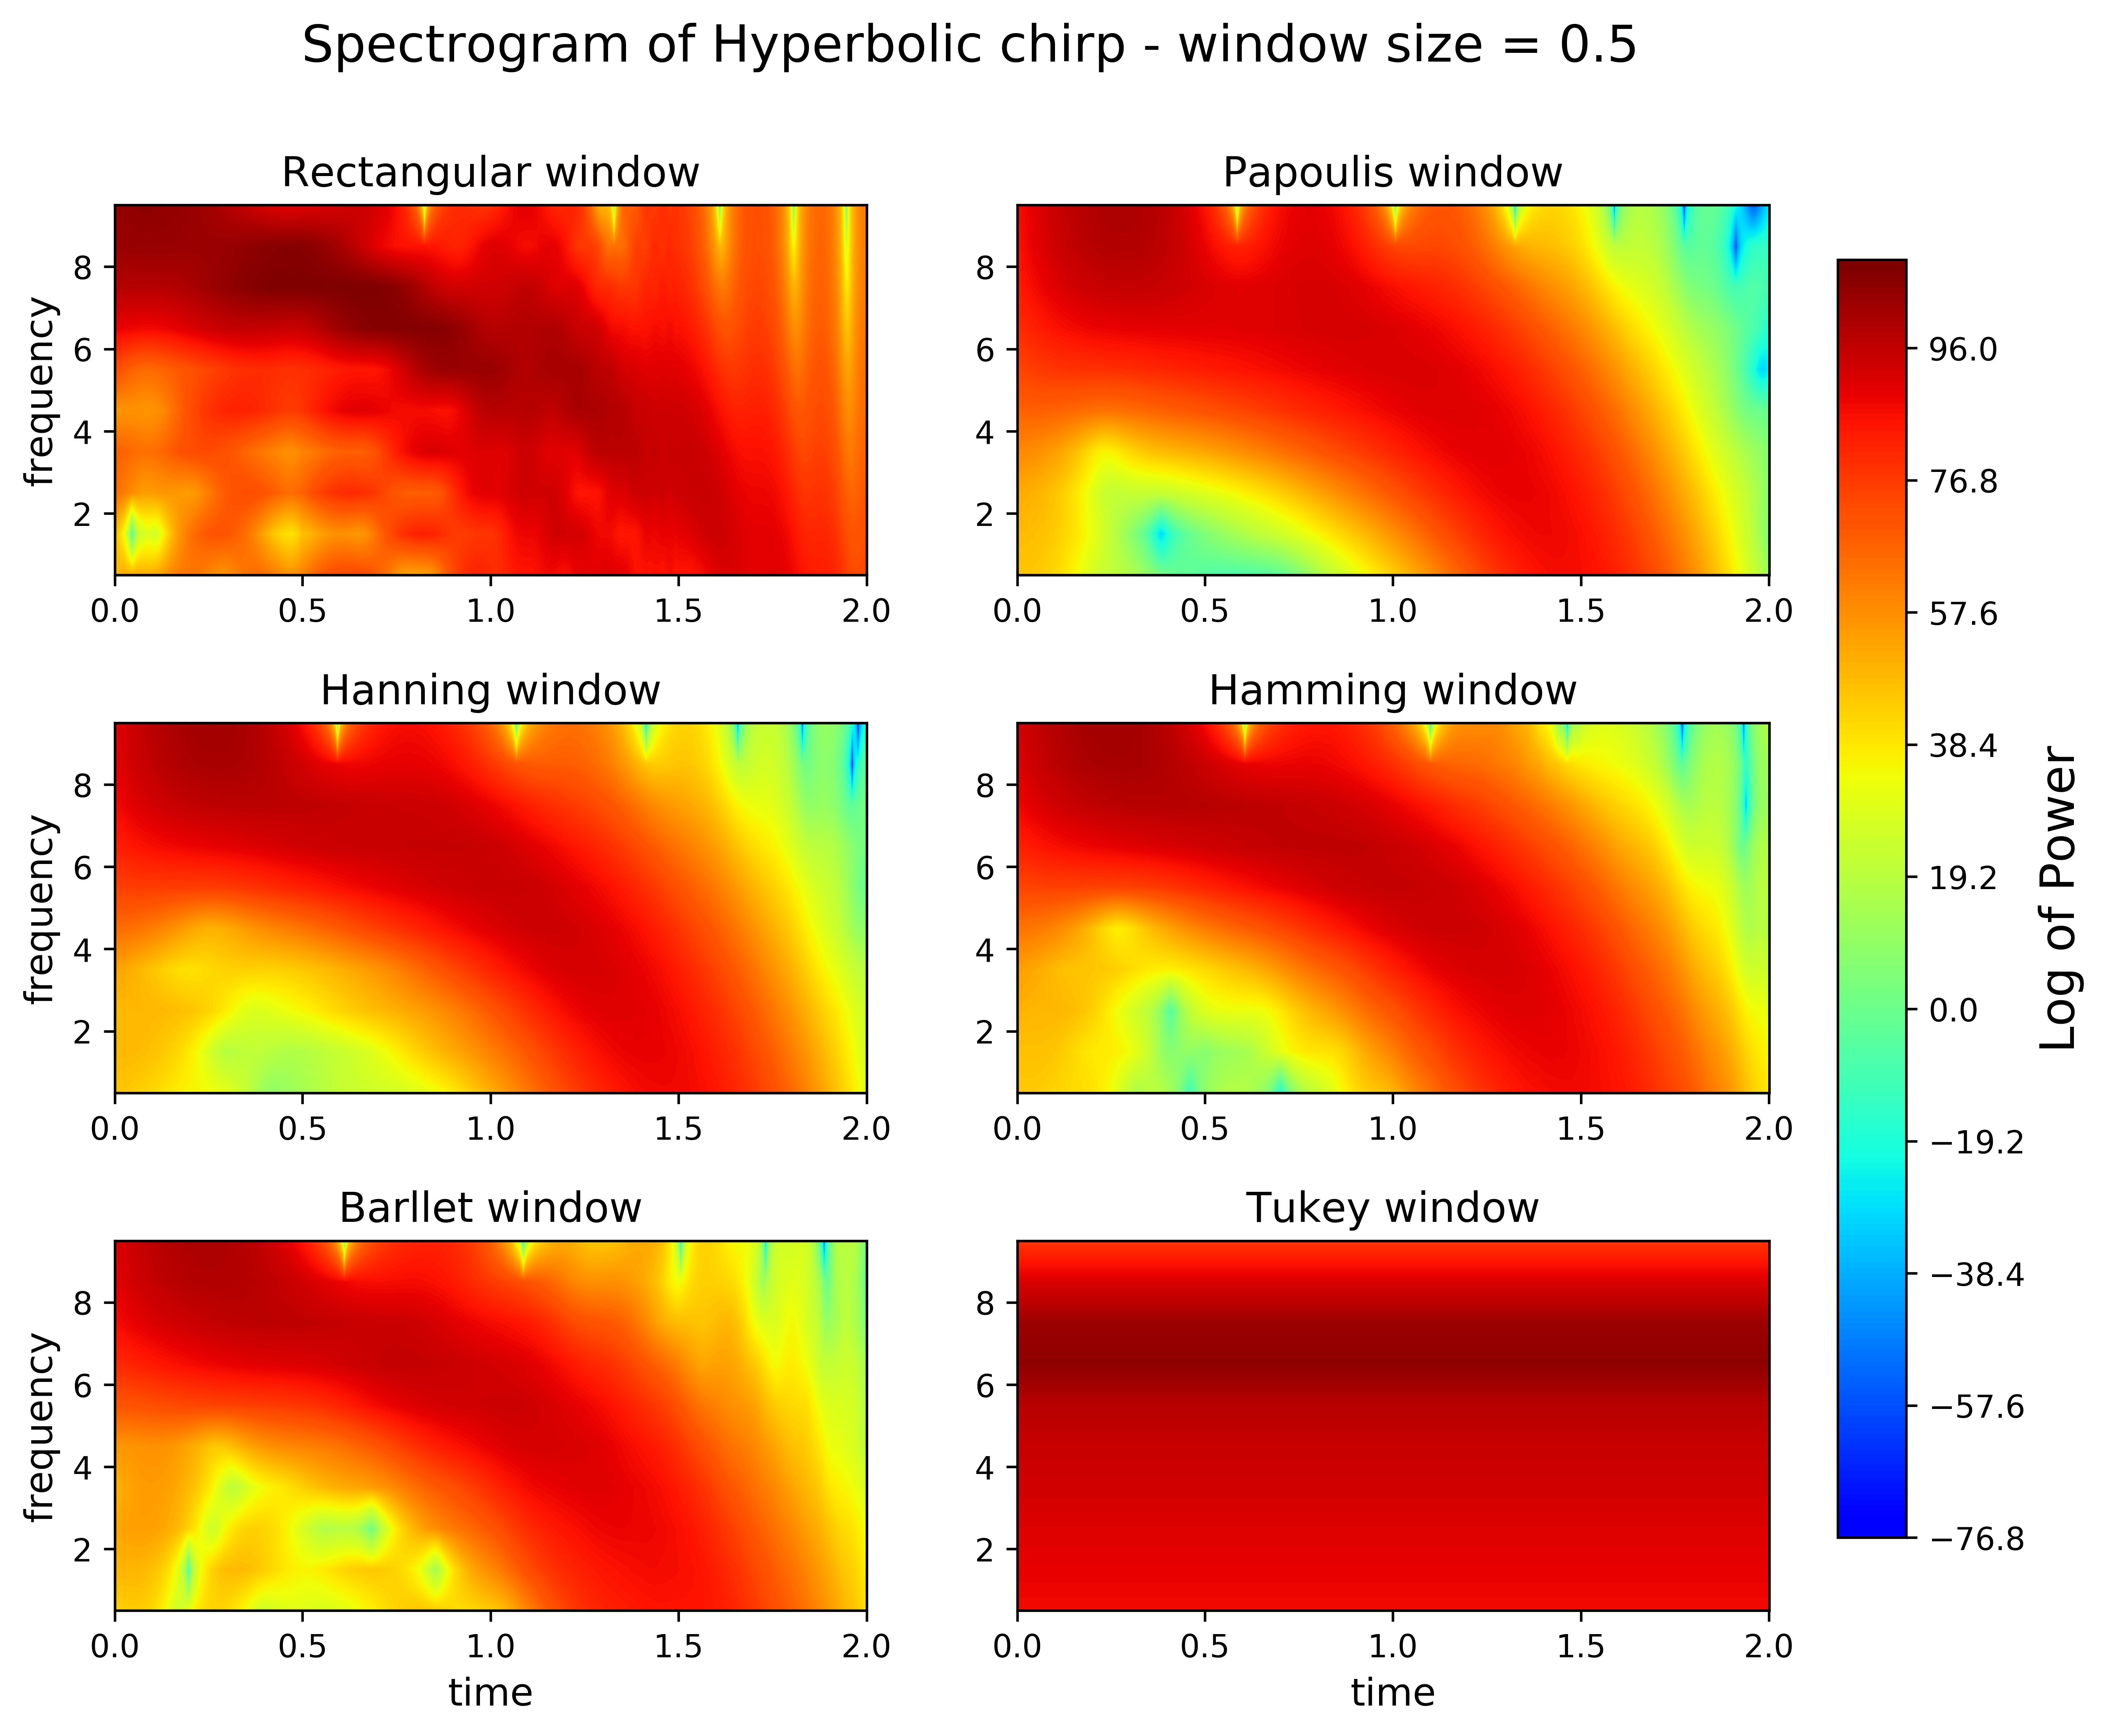
\includegraphics{../scripts/exercicio2/espectros/Hyperbolic_ws0.5.jpg}}	
	\end{center}
	\vspace{1mm}
	\label{ex1_fig1}
\end{figure}

Espectrogramas do \textbf{chirp hiperbólico}, $0 \leq t \leq 6$ e tamanho das janelas = 0.1: Figura 2.15.

% FIGURA
\begin{figure}[ht!]
	\legenda{Figura 2.15: Espectrogramas do chirp hiperbólico com janelas de tamanho igual a 0.1. Comparar com última linha da Figura 1.3.}
	\vspace{3mm}	
	\begin{center}
		\resizebox{\textwidth}{!}{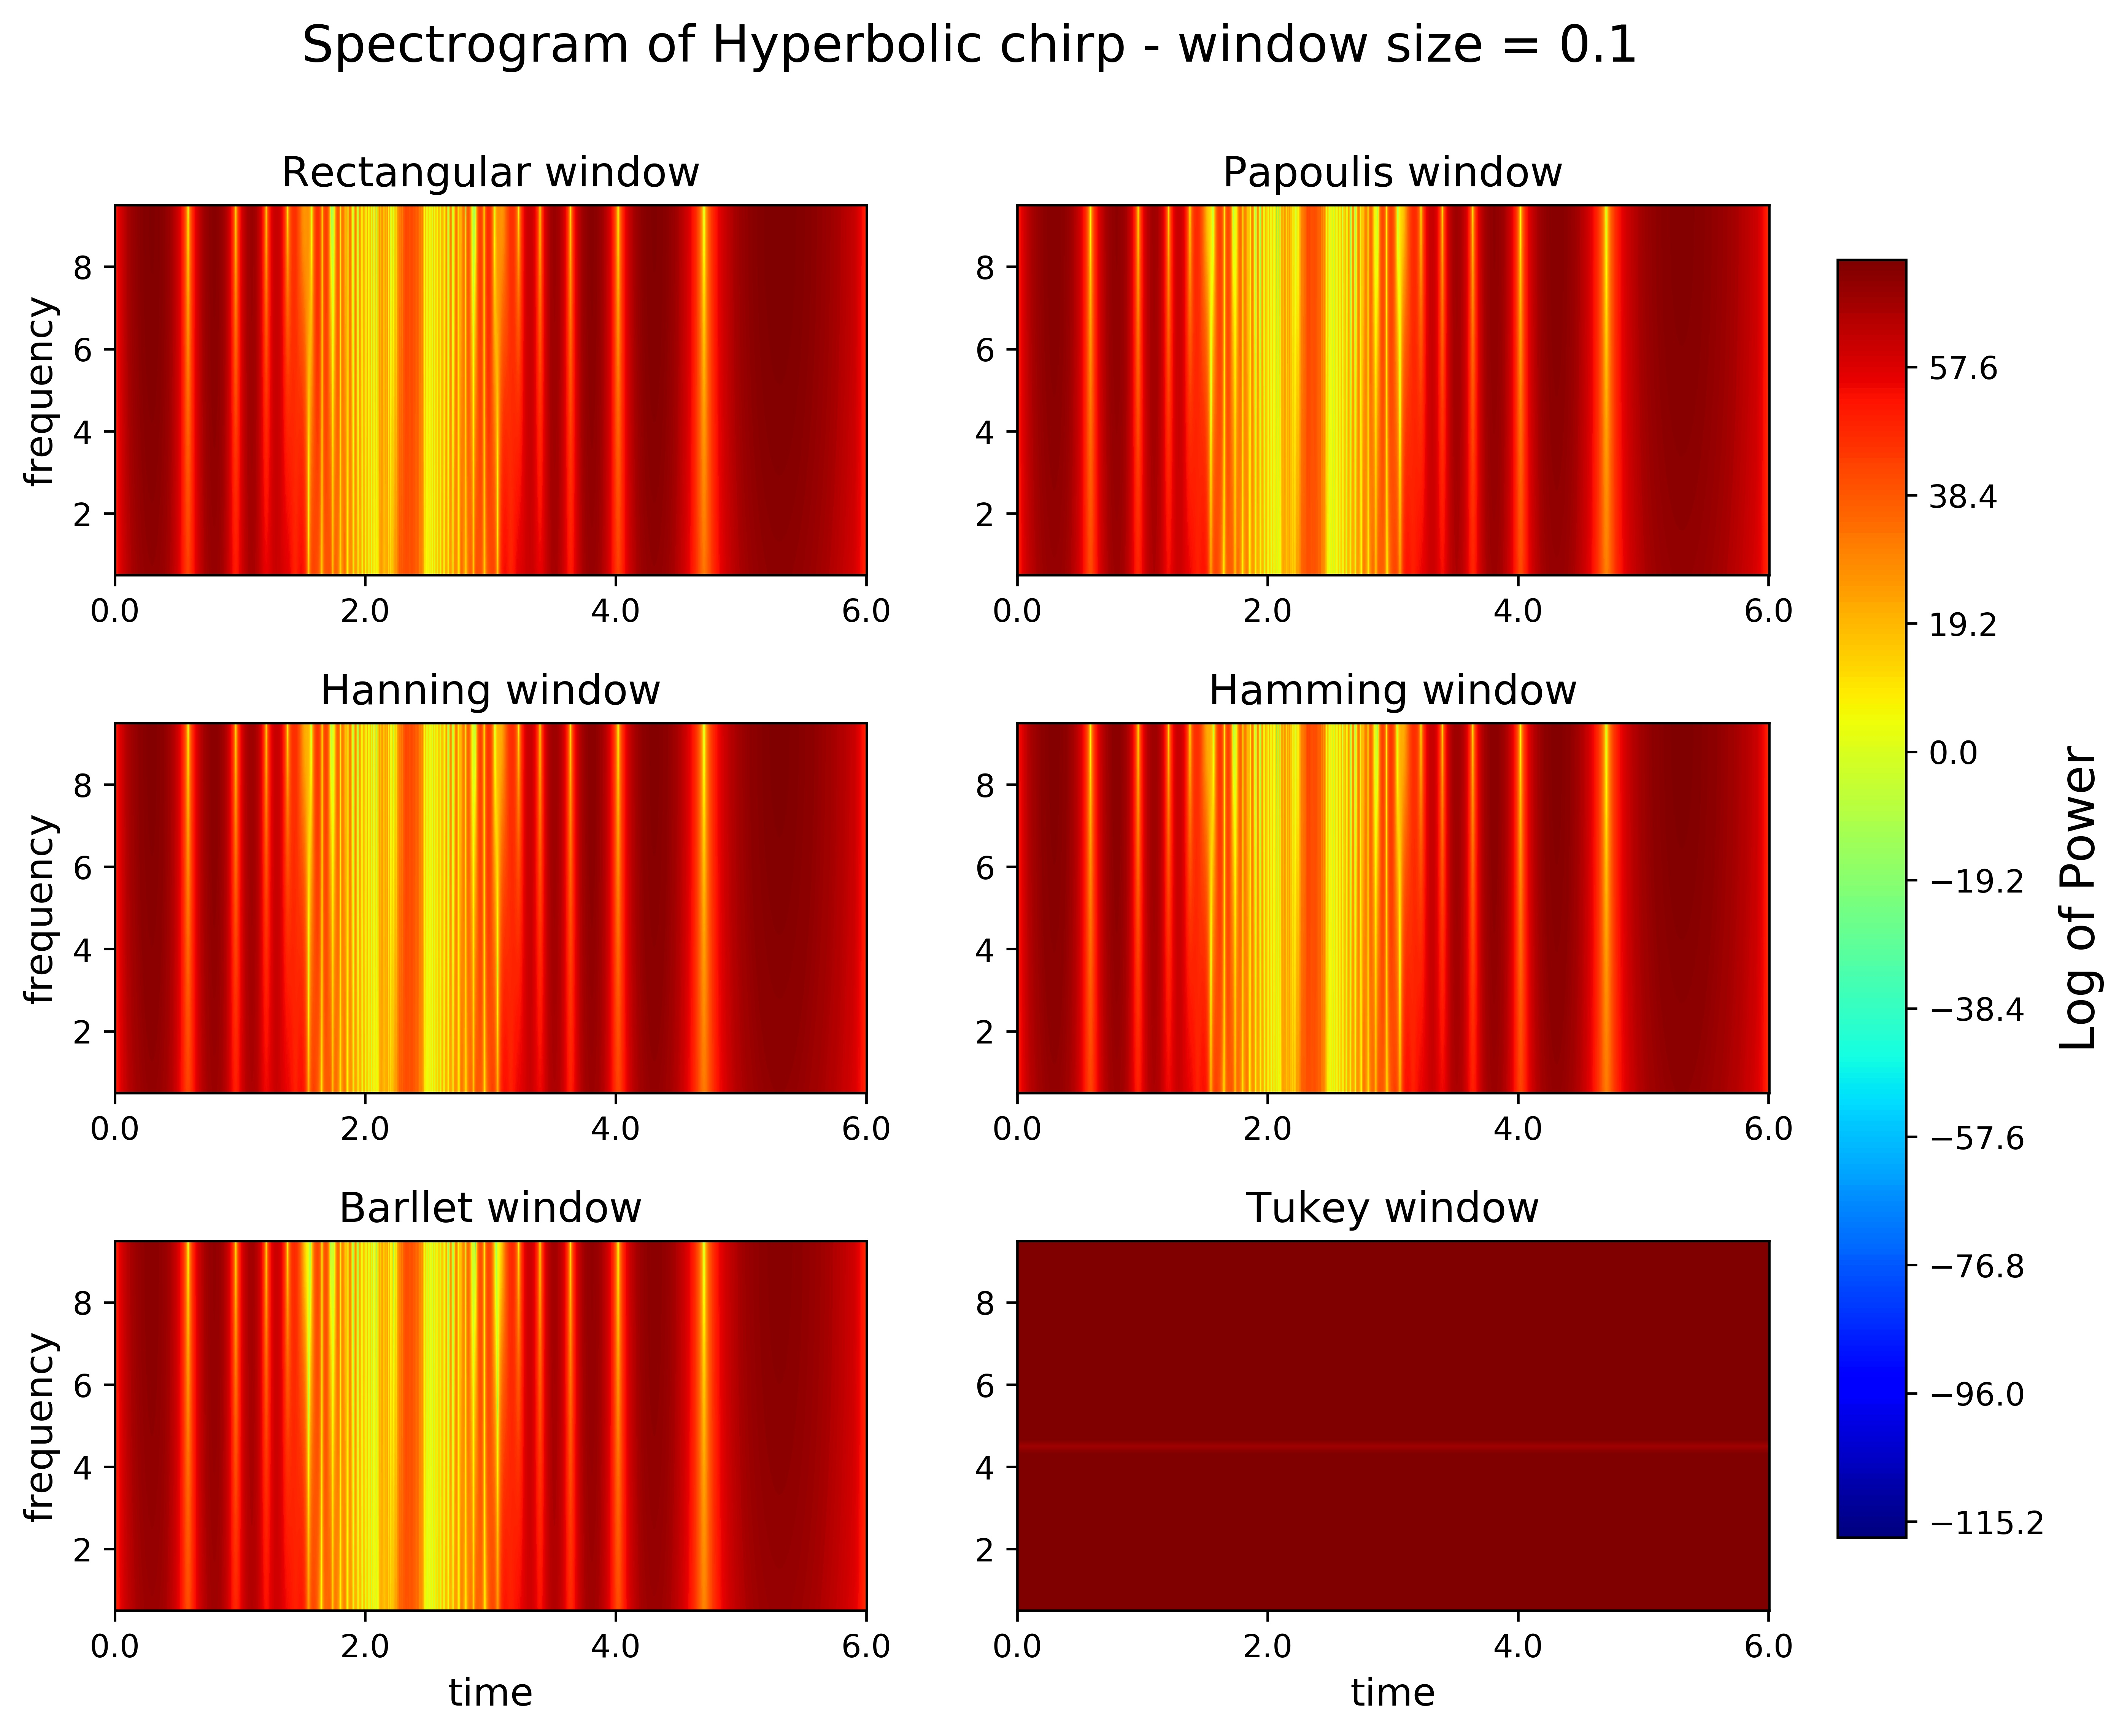
\includegraphics{../scripts/exercicio2/espectros/TEST_Hyperbolic_ws0.1.jpg}}	
	\end{center}
	\vspace{1mm}
	\label{ex1_fig1}
\end{figure}


Espectrogramas do \textbf{chirp hiperbólico}, $0 \leq t \leq 6$ e tamanho das janelas = 0.5: Figura 2.16.

% FIGURA
\begin{figure}[ht!]
	\legenda{Figura 2.16: Espectrogramas do chirp hiperbólico com janelas de tamanho igual a 0.5. Comparar com última linha da Figura 1.3.}
	\vspace{3mm}	
	\begin{center}
		\resizebox{\textwidth}{!}{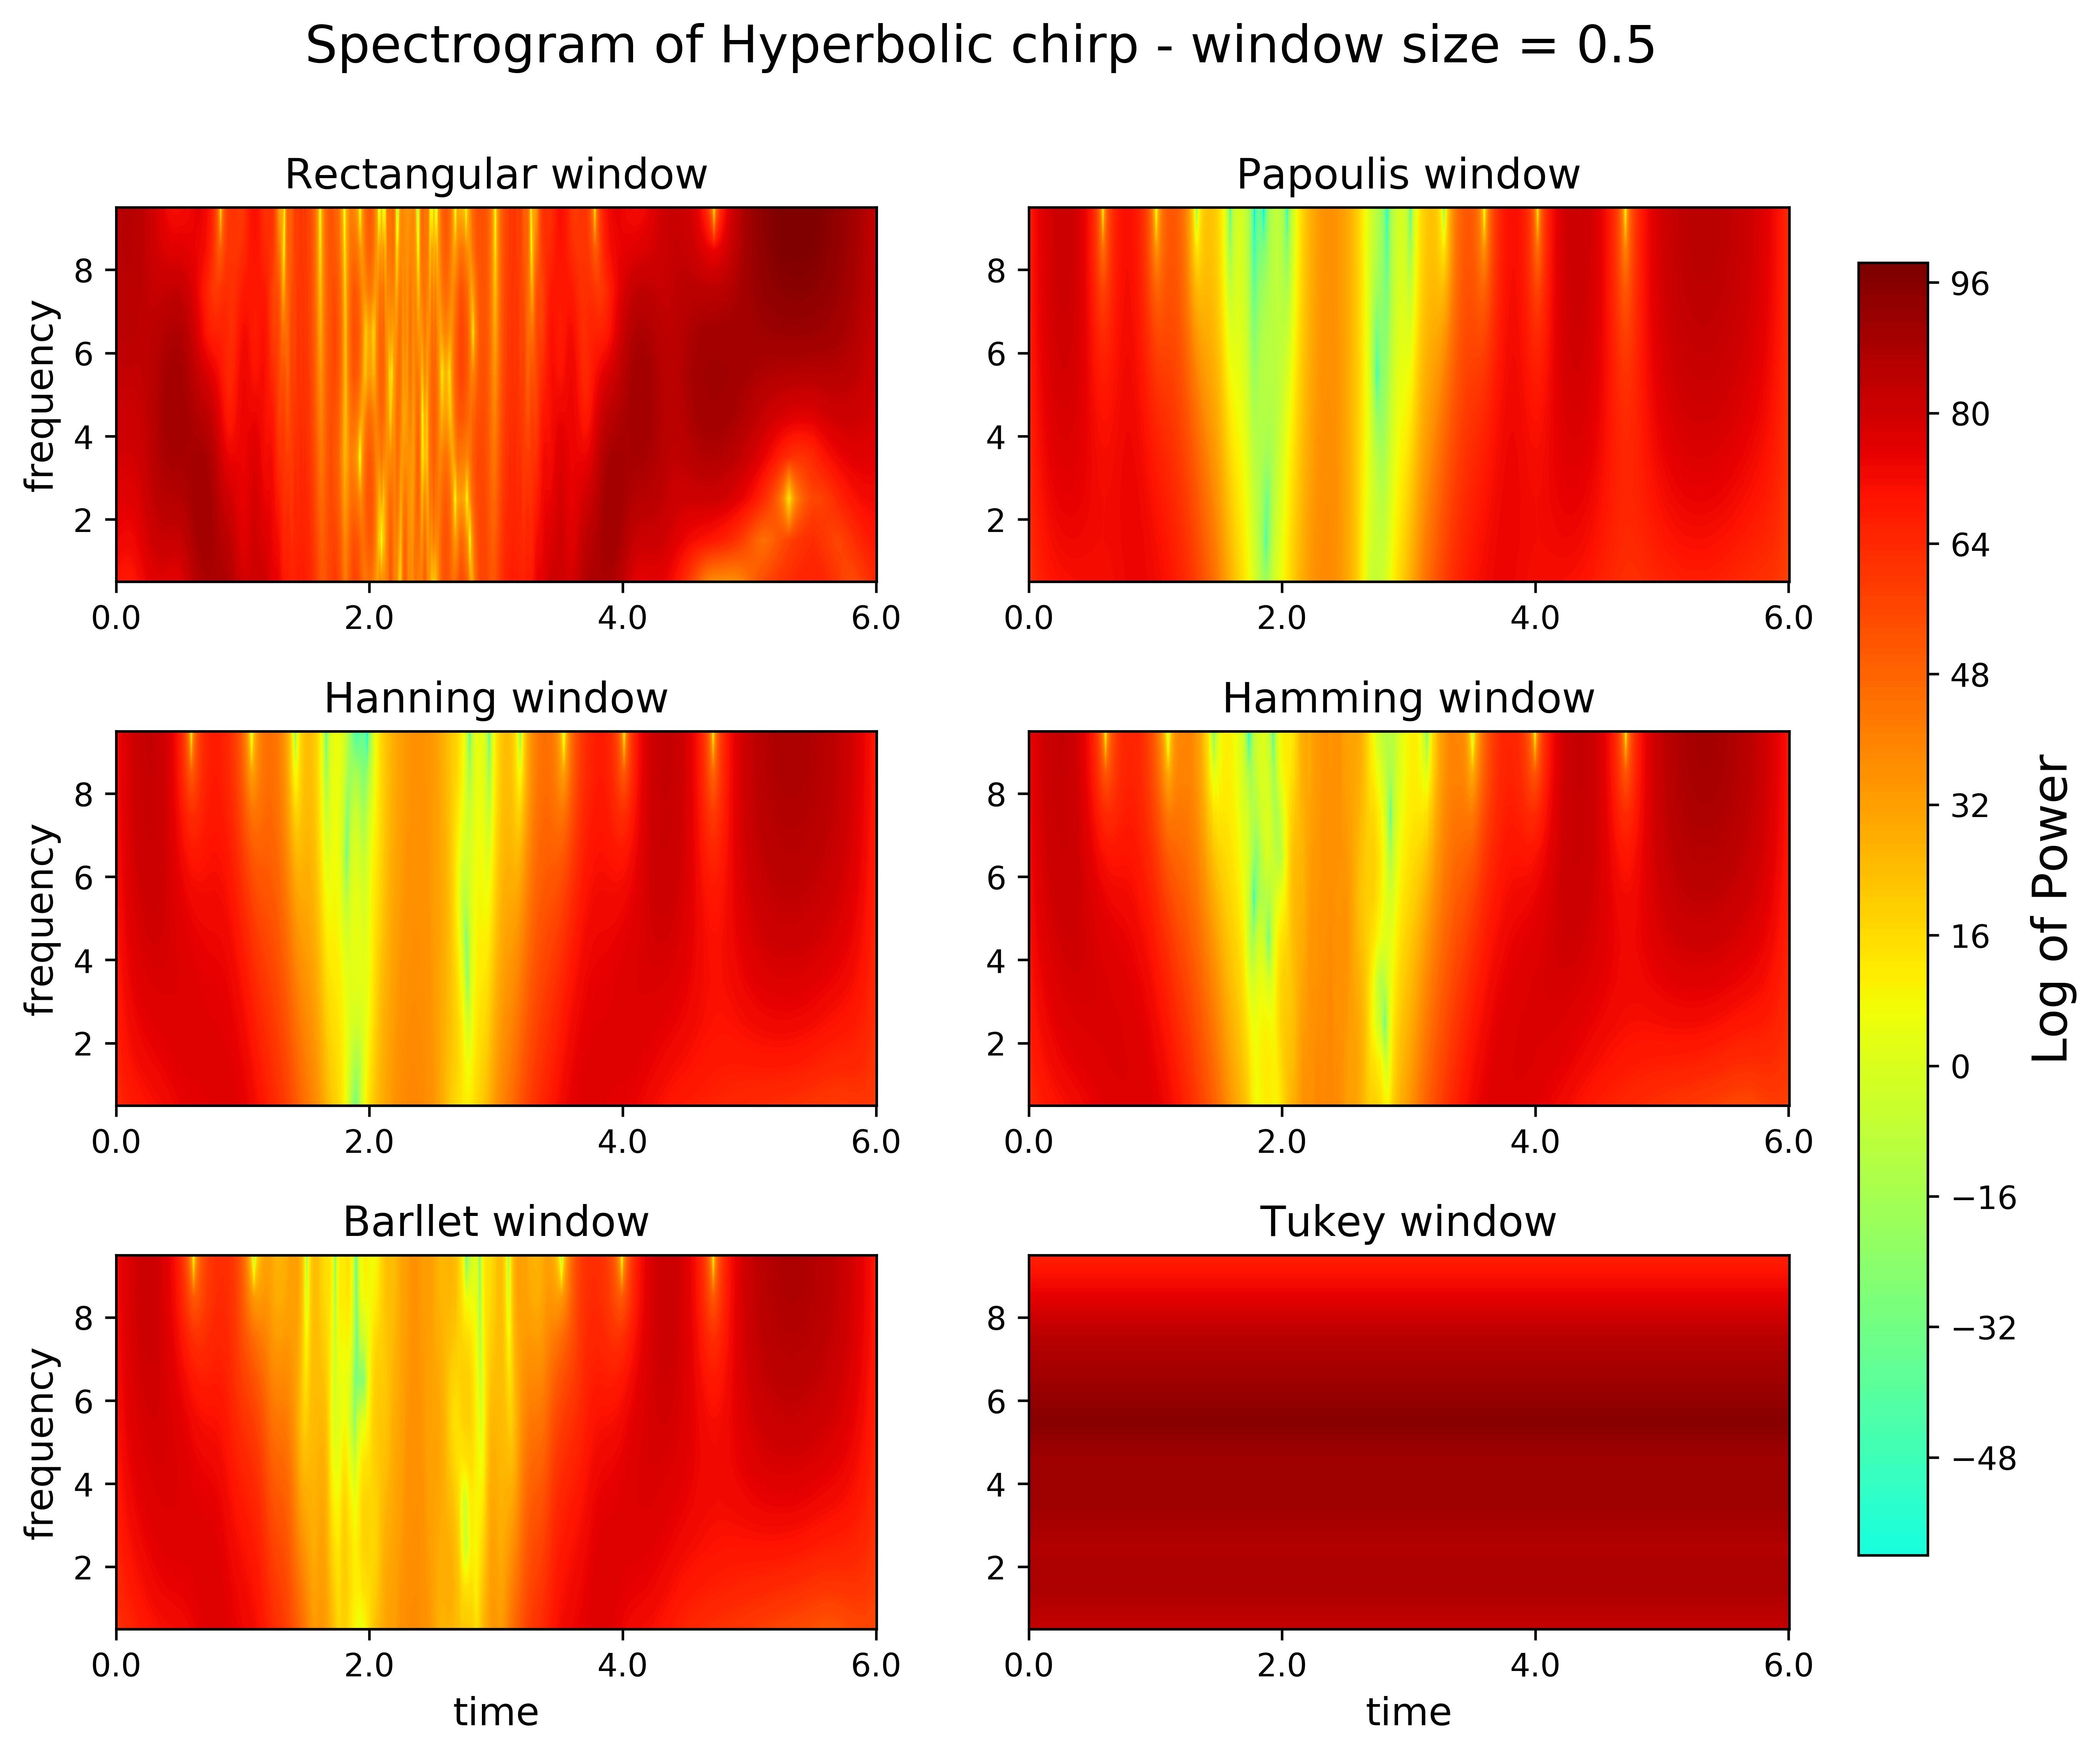
\includegraphics{../scripts/exercicio2/espectros/TEST_Hyperbolic_ws0.5.jpg}}	
	\end{center}
	\vspace{1mm}
	\label{ex1_fig1}
\end{figure}

%%%%%%%%%%%%%%%%%%%%%%%%%%%%%%%%%%%%%%%%%%%%%%%%%%%%%%%%%% 2.c

\subsection*{2.c} 
\addcontentsline{toc}{section}{\protect\numberline{} 2.c}%

Se o objetivo da análise é obter detalhes da variação das diferentes frequências do sinal ao longo do tempo, a implementação das WFT com janelas grandes é desejada, uma vez que isso oferecerá maior resolução frequencial no espectrograma. Para o chirp gaussiano, uma vez que a variação da frequência é suave e com poucos componentes, as janelas de tamanho 0.1 e 0.5 (Figuras 2.4, 2.5 e 2.6) foram equivalentes em resultado. 

Já para o chirp linear, a janela de tamanho igual a 0.1 não foi capaz de captar a variação linear (e suave) da frequência (Figura 2.7). As janelas de tamanho 0.5 conseguiram. %Em particular, na Figura 2.8 somente a janela retangular captou bem a variação da frequência. Isso pode ser explicado pela Figura 2.1, que ilustra a transformada da janela retangular como tendo a menor largura (em frequência) e, portanto, melhor resolução frequencial. %Em contrapartida, a Figura 2.4 ilustra que todas as transformadas possuem larga distribuição, ou seja, baixíssima resolução.

%Em particular, na Figura 2.8 somente a janela retangular captou bem a variação da frequência. Isso pode ser explicado pela Figura 2.1, que ilustra a transformada da janela retangular como tendo a menor largura (em frequência) e, portanto, melhor resolução frequencial. 
As Figuras 2.10 e 2.11 (chirp quadrático), quando contrastadas, também ilustram a incapacidade das janelas de tamanho igual a 0.1 de contribuir para a análise deste chirp. Na Figura 2.10, assim como na Figura 2.7, somente a janela retangular foi capaz de captar uma variação apreciável de frequência. Isso pode ser explicado pela Figura 2.1, que ilustra a transformada da janela retangular como tendo a menor largura (em frequência) e, portanto, melhor resolução frequencial. %As Figuras 2.11 e 2.12 atestam a variação quadrática da frequência do chirp analisado com o tempo.

O chirp hiperbólico foi o sinal que melhor ilustrou o \textit{trade-off} da resolução tempo $\times$ frequência por trás da definição do tamanho da janela. As Figuras 2.13 e 2.15 exibem os espectrogramas para as janelas de tamanho igual a 0.1, ou seja, de alta resolução temporal. A variação das cores (das frequências) na direção do eixo horizontal nestas figuras é bem acentuada. A WFT com estas janelas captou bem a variação temporal do sinal sem determinar bem quais frequências compõem o sinal localmente. Em contrapartida, nas Figura 2.14 e 2.16 o tamanho das janelas é 0.5, ou seja, a resolução temporal é menor. Com isso, o espectrograma exibe forte variação de cores que resulta da melhor representação de frequências, ganhando resolução vertical ao passo que perde a capacidade de descrever a variação horizontal dessas cores como antes. 

Em conjunto, as figuras desta seção atestam a capacidade da WFT de analisar conteúdos frequenciais de um sinal localmente, conferindo uma componente extra de análise: o tempo. Este componente é ausente na análise de Fourier tradicional, que possui um caráter global de análise. Com a WFT surgem parâmetros relevantes à nossa análise desde a análise de Fourier, a saber, o tamanho da função janela escolhida, diretamente relacionado ao já conhecido princípio da incerteza. Quanto maior (menor) a largura da janela, menor (maior) será a resolução temporal da ferramenta e maior (menor) será sua resolução frequencial. Por fim, outro importante parâmetro da WFT é a função janela em si, uma vez que os resultados deste exercício sugerem que, em alguns casos, algumas funções janela são mais úteis que outras em captar as diferentes frequências de um sinal.
















